\begin{figure}[htbp]
\centering
\setlength{\tabcolsep}{1pt}
\begin{tabular}{cc}
\subf{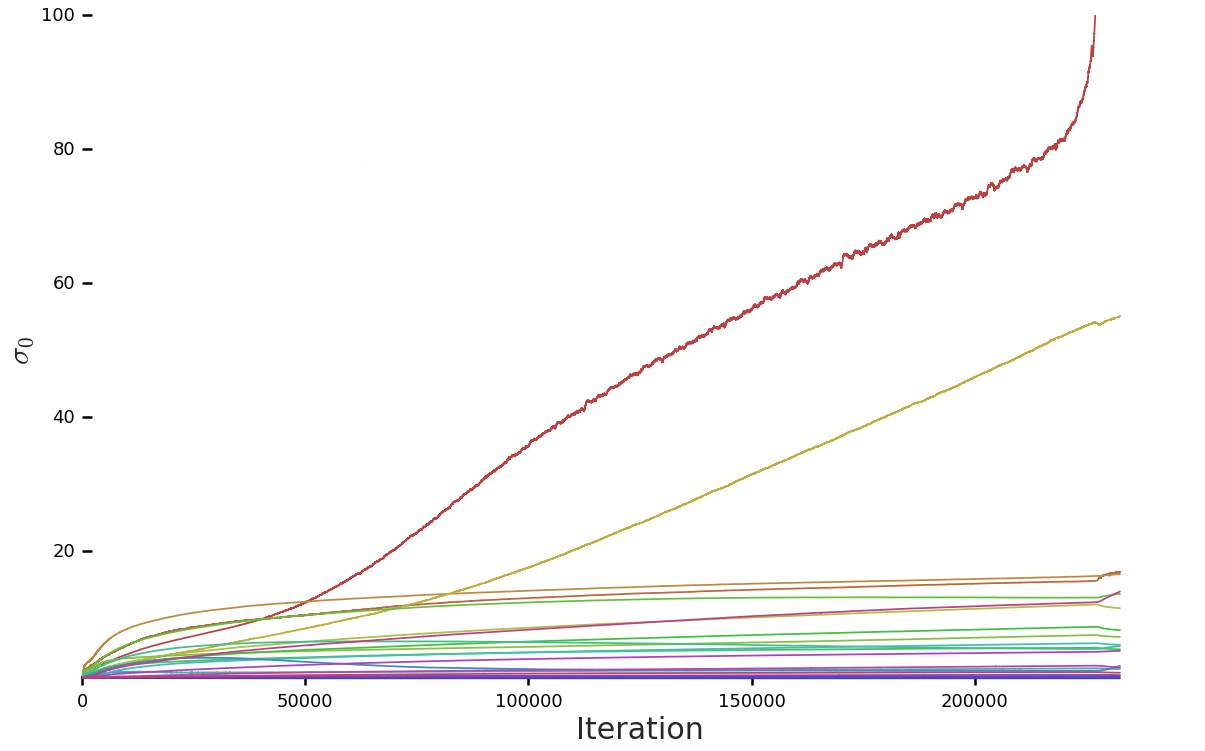
\includegraphics[width=0.48\textwidth]{images/1535537/GSV0.jpg}}{(a) \gen{} $\sigma_0$ } & 
\subf{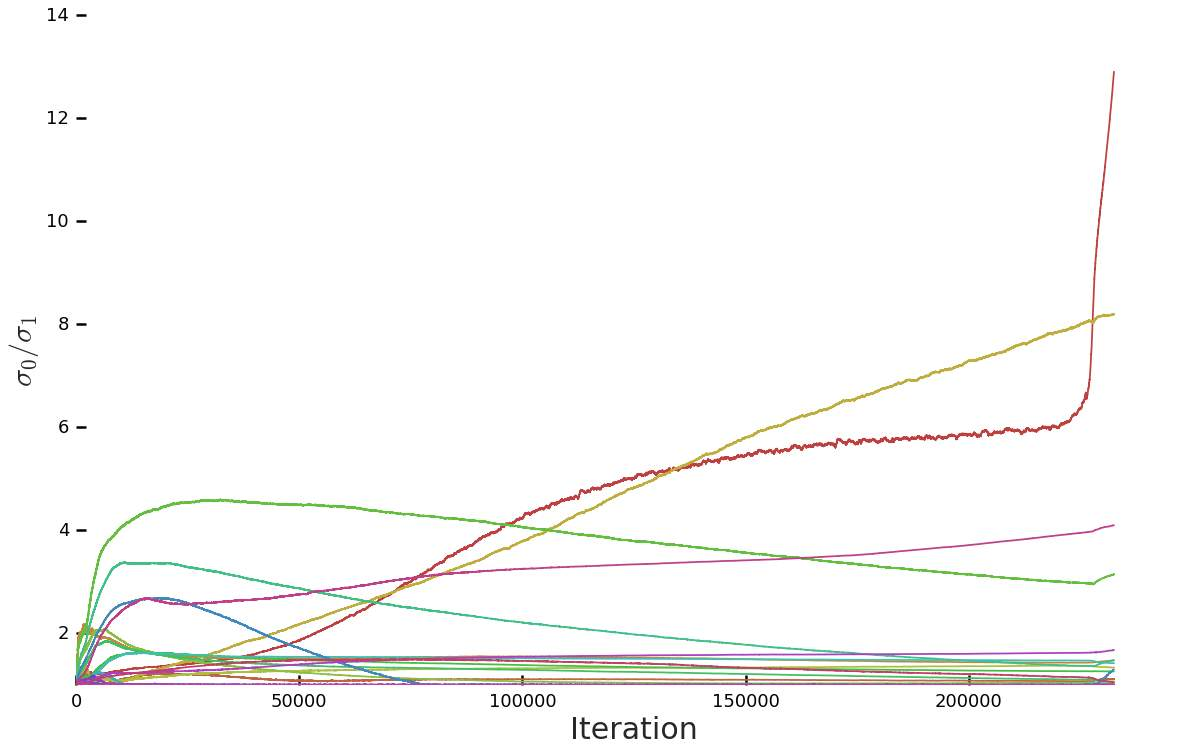
\includegraphics[width=0.48\textwidth]{images/1535537/GSVR.jpg}}{(b) \gen{} $\frac{\sigma_0}{\sigma_1}$ } \\
\subf{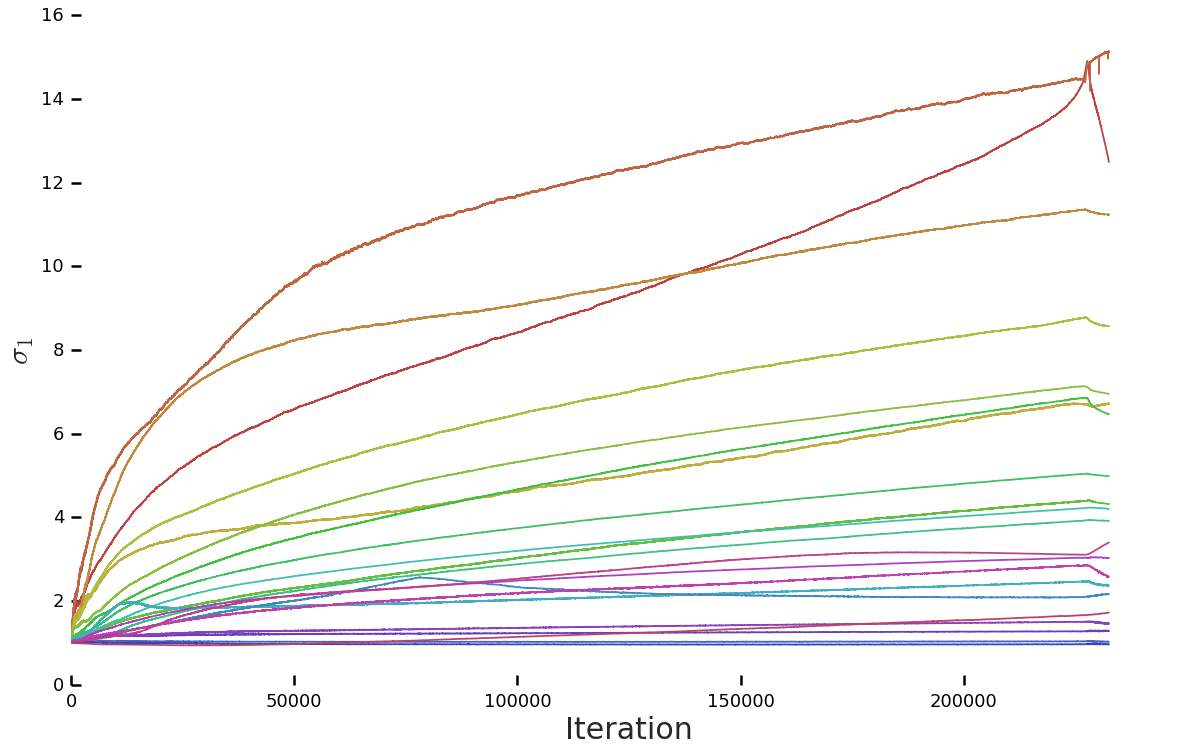
\includegraphics[width=0.48\textwidth]{images/1535537/GSV1.jpg}}{(c) \gen{} $\sigma_1$} & 
\subf{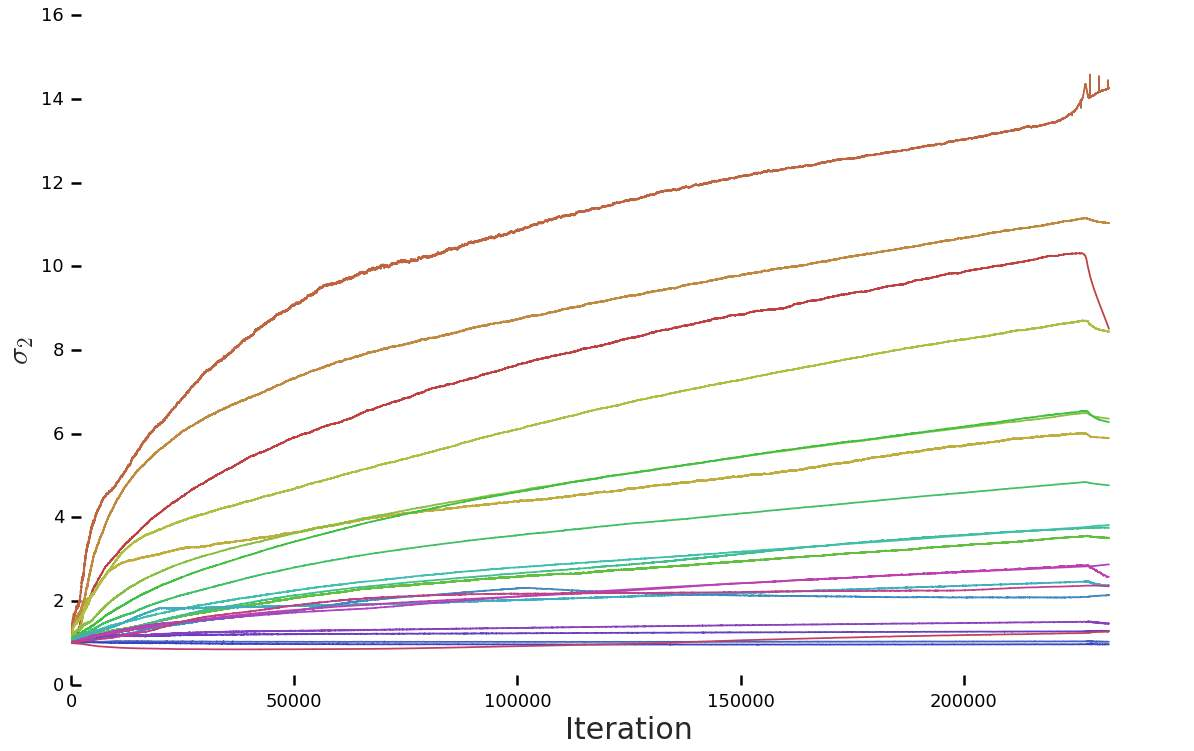
\includegraphics[width=0.48\textwidth]{images/1535537/GSV2.jpg}}{(d) \gen{} $\sigma_2$} \\
\subf{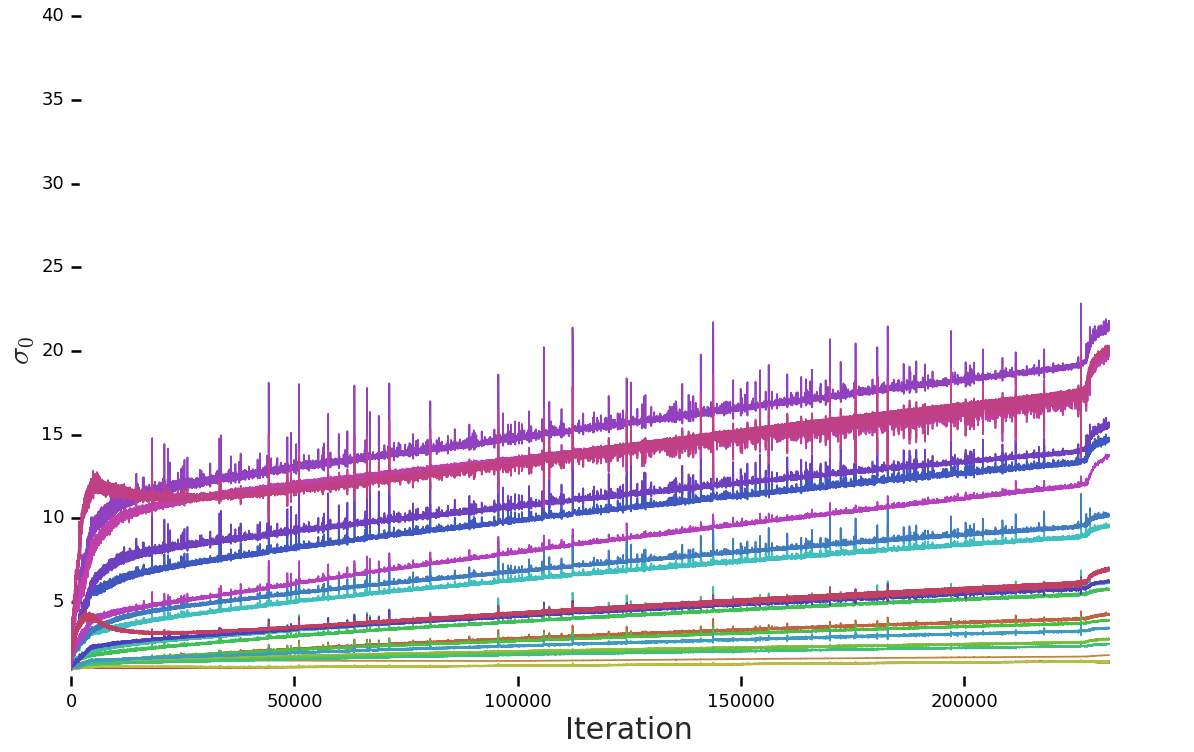
\includegraphics[width=0.48\textwidth]{images/1535537/DSV0.jpg}}{(e) \discr{} $\sigma_0$ } & 
\subf{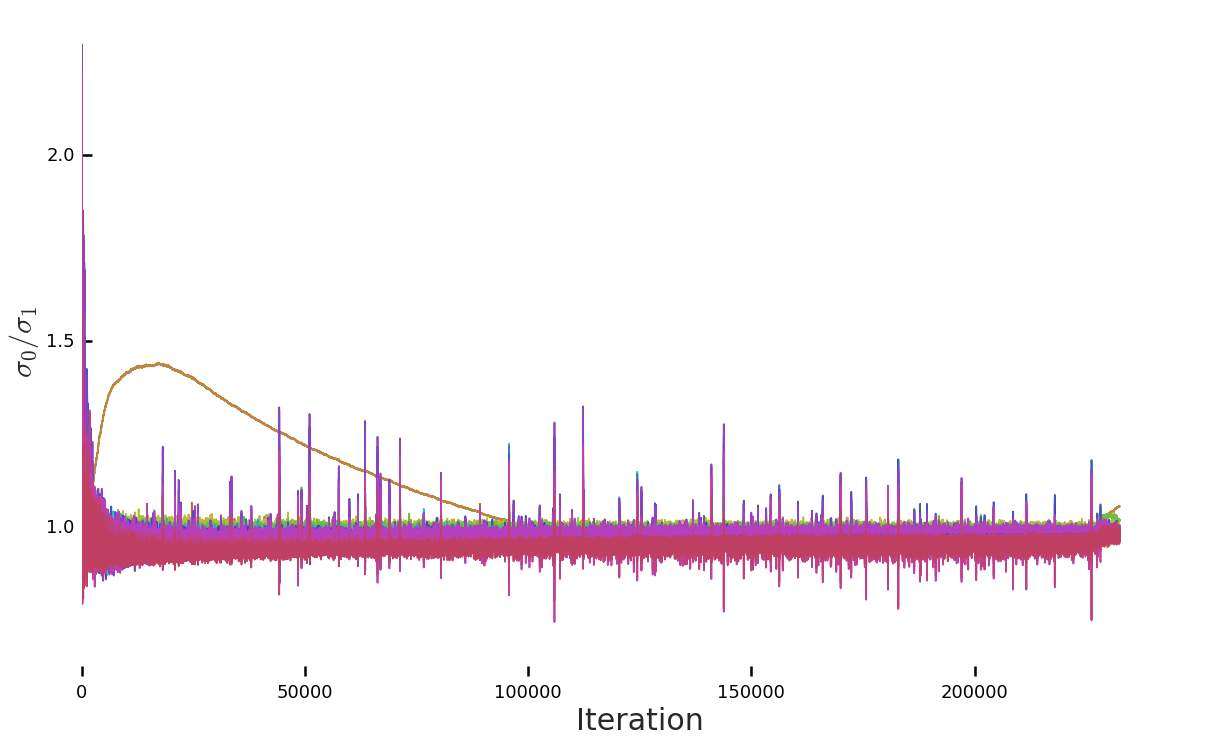
\includegraphics[width=0.48\textwidth]{images/1535537/DSVR.jpg}}{(f) \discr{} $\frac{\sigma_0}{\sigma_1}$ } \\
\subf{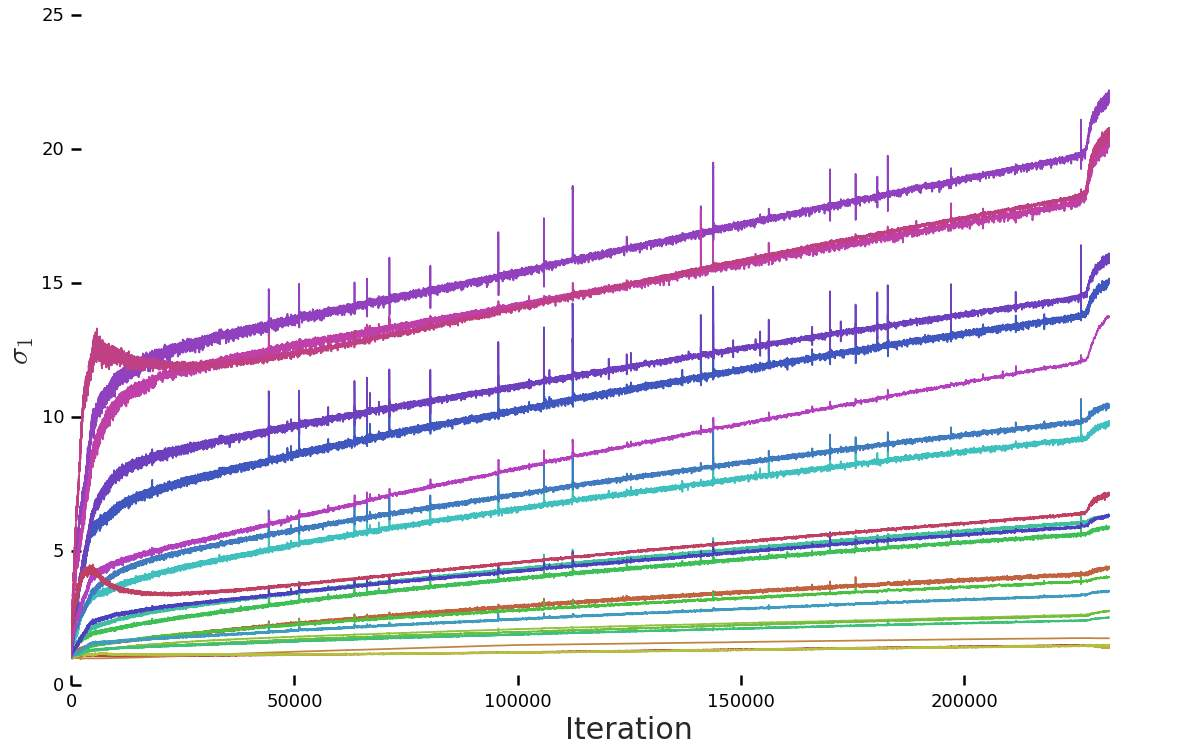
\includegraphics[width=0.48\textwidth]{images/1535537/DSV1.jpg}}{(g) \discr{} $\sigma_1$} & 
\subf{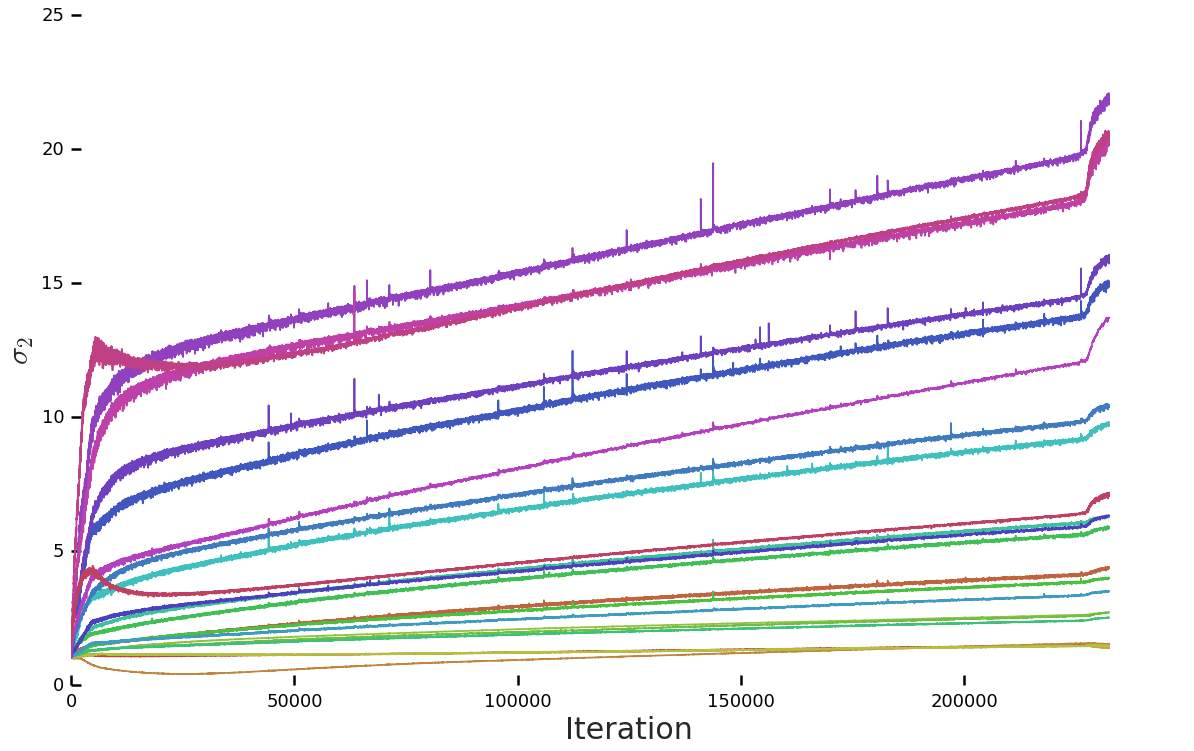
\includegraphics[width=0.48\textwidth]{images/1535537/DSV2.jpg}}{(h) \discr{} $\sigma_2$} 
\end{tabular}
\caption{Training statistics for a typical model without special modifications. Collapse occurs after 200000 iterations.}
\label{GD_spectra_unreg}
\end{figure}


% Reg sigma bois
\begin{figure}[htbp]
\centering
\setlength{\tabcolsep}{1pt}
\begin{tabular}{cc}
\subf{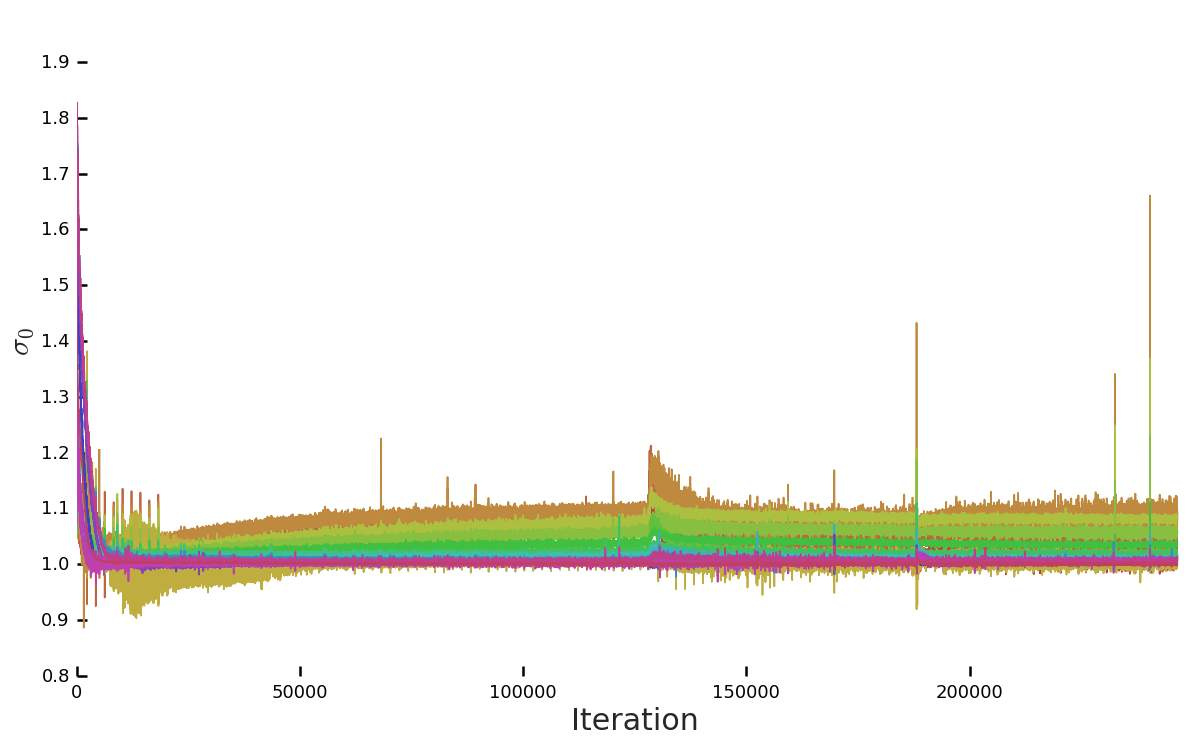
\includegraphics[width=0.48\textwidth]{images/1506681_GSR2_1/GSV0.jpg}}{(a) $\sigma_0$ } & 
\subf{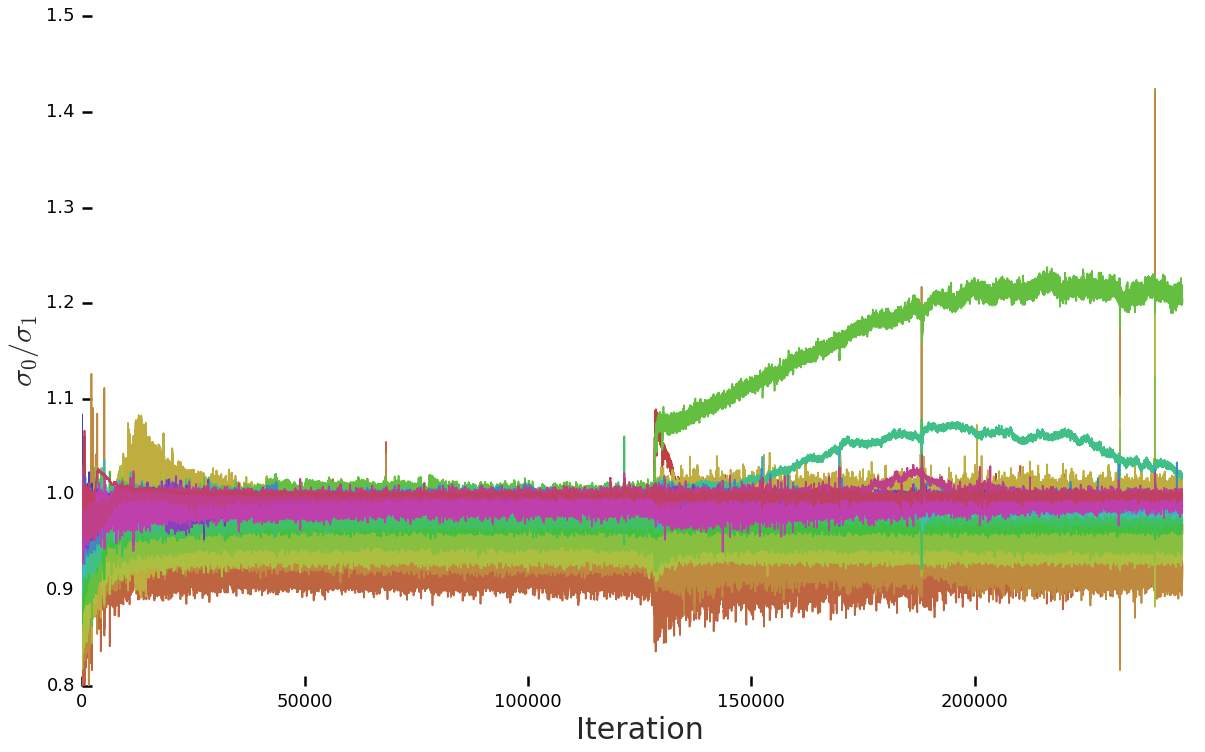
\includegraphics[width=0.48\textwidth]{images/1506681_GSR2_1/GSVR.jpg}}{(b) $\frac{\sigma_0}{\sigma_1}$ } \\
\subf{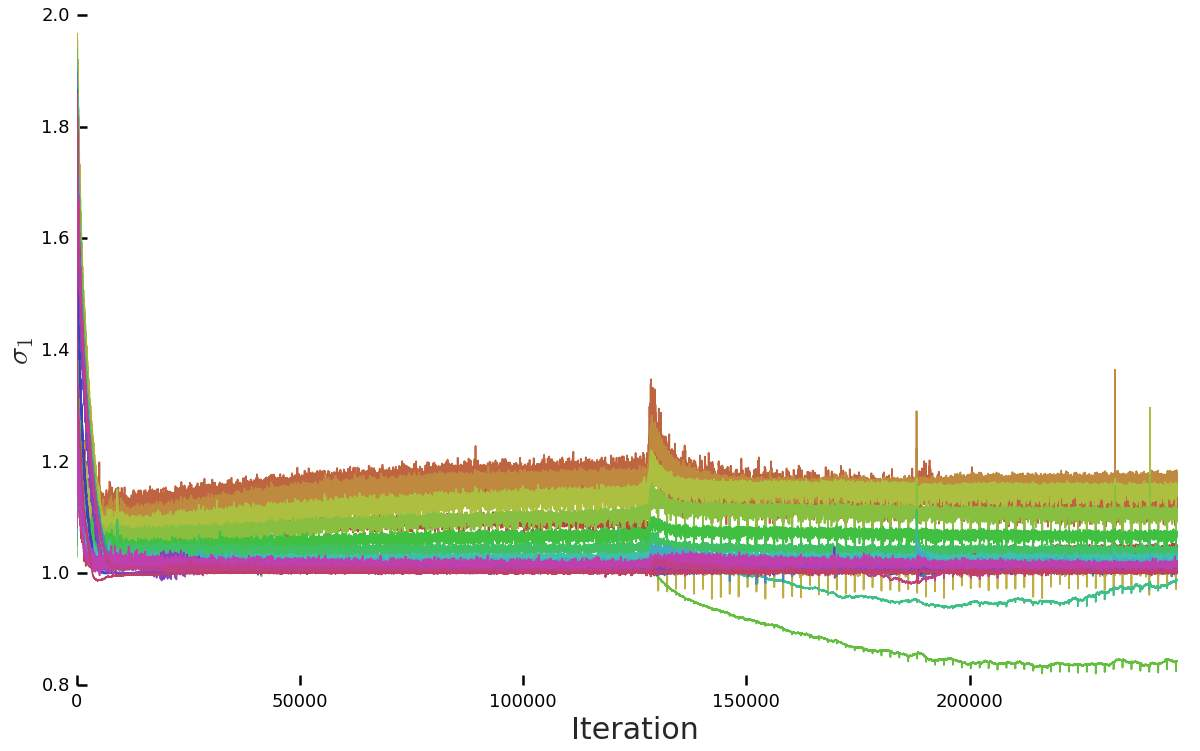
\includegraphics[width=0.48\textwidth]{images/1506681_GSR2_1/GSV1.jpg}}{(c) $\sigma_1$} & 
\subf{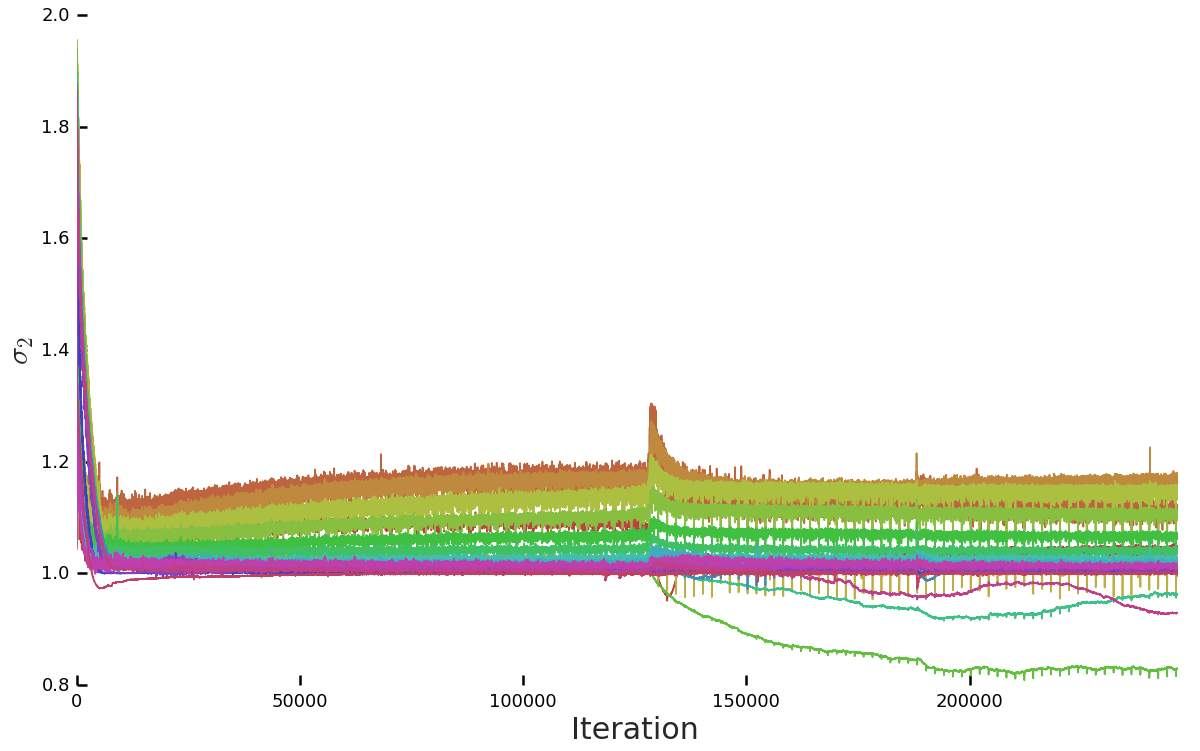
\includegraphics[width=0.48\textwidth]{images/1506681_GSR2_1/GSV2.jpg}}{(d) $\sigma_2$}\\
\end{tabular}
\caption{\gen{} training statistics with $\sigma_0$ in \gen{} regularized towards 1. Collapse occurs after 125000 iterations.}
\label{G_spectra_regsigma}
\end{figure}

\begin{figure}[htbp]
\centering
\setlength{\tabcolsep}{1pt}
\begin{tabular}{cc}
\subf{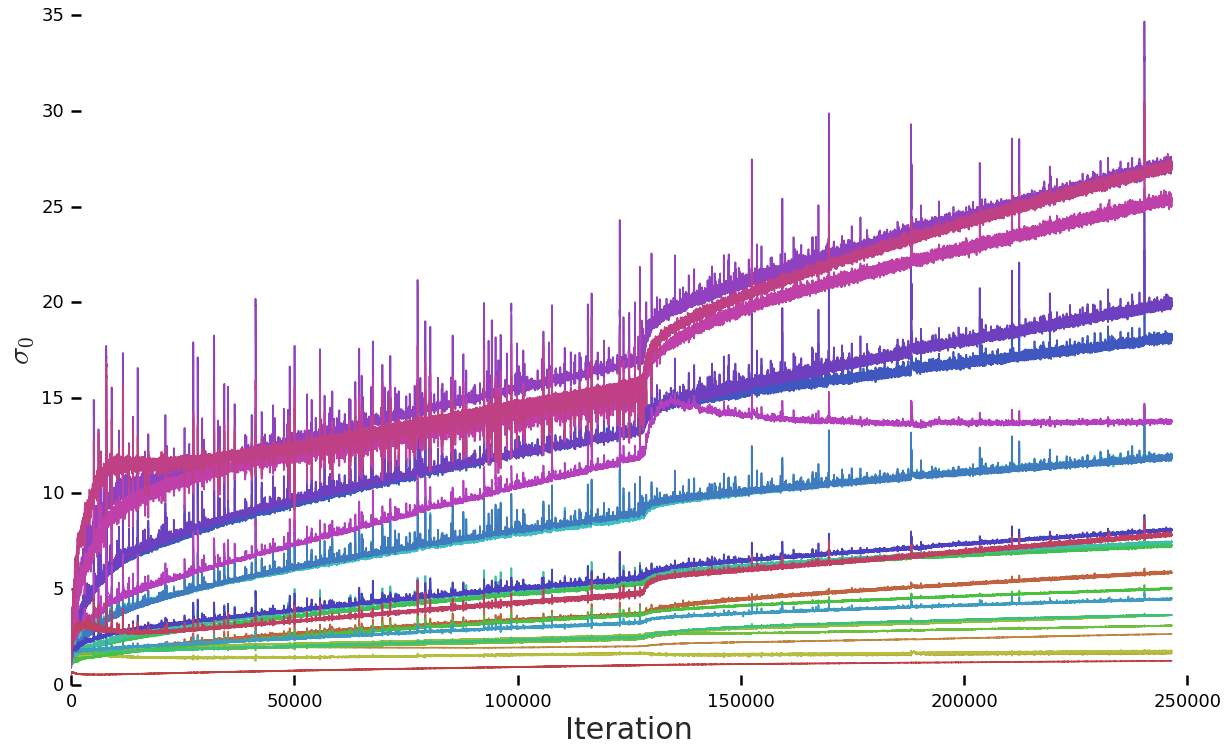
\includegraphics[width=0.48\textwidth]{images/1506681_GSR2_1/DSV0.jpg}}{(a) $\sigma_0$ } & 
\subf{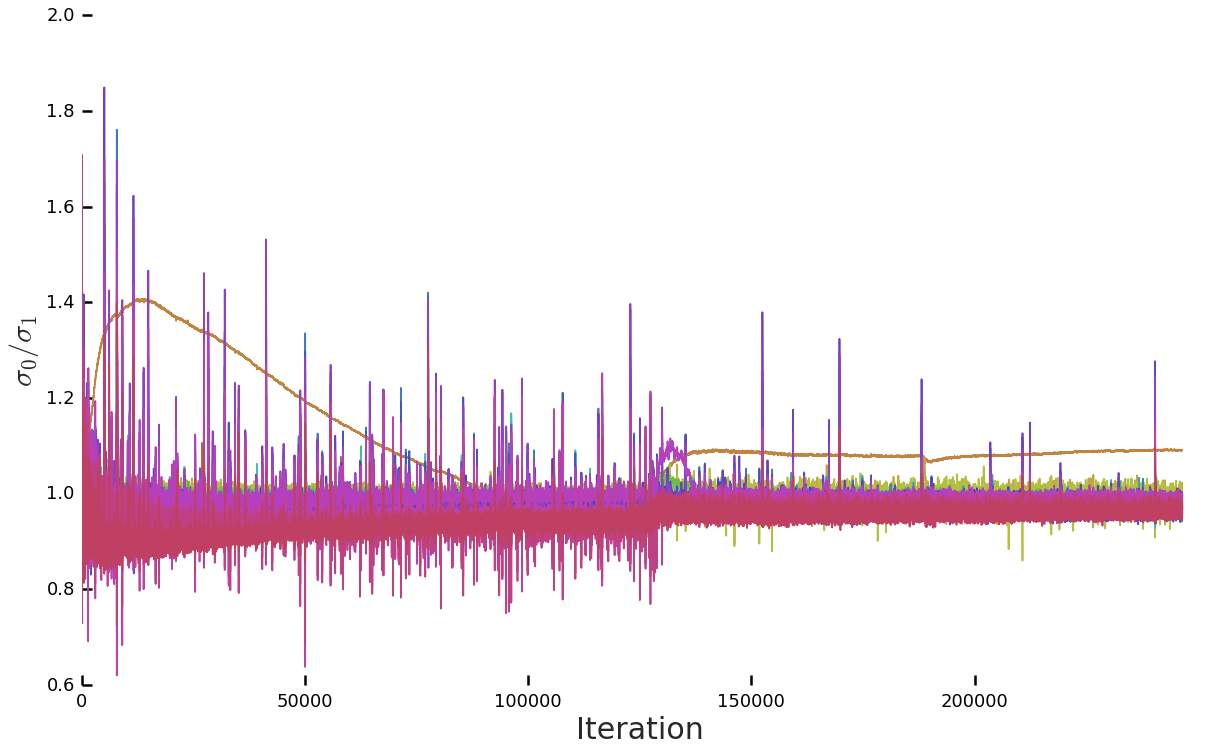
\includegraphics[width=0.48\textwidth]{images/1506681_GSR2_1/DSVR.jpg}}{(b) $\frac{\sigma_0}{\sigma_1}$ } \\
\subf{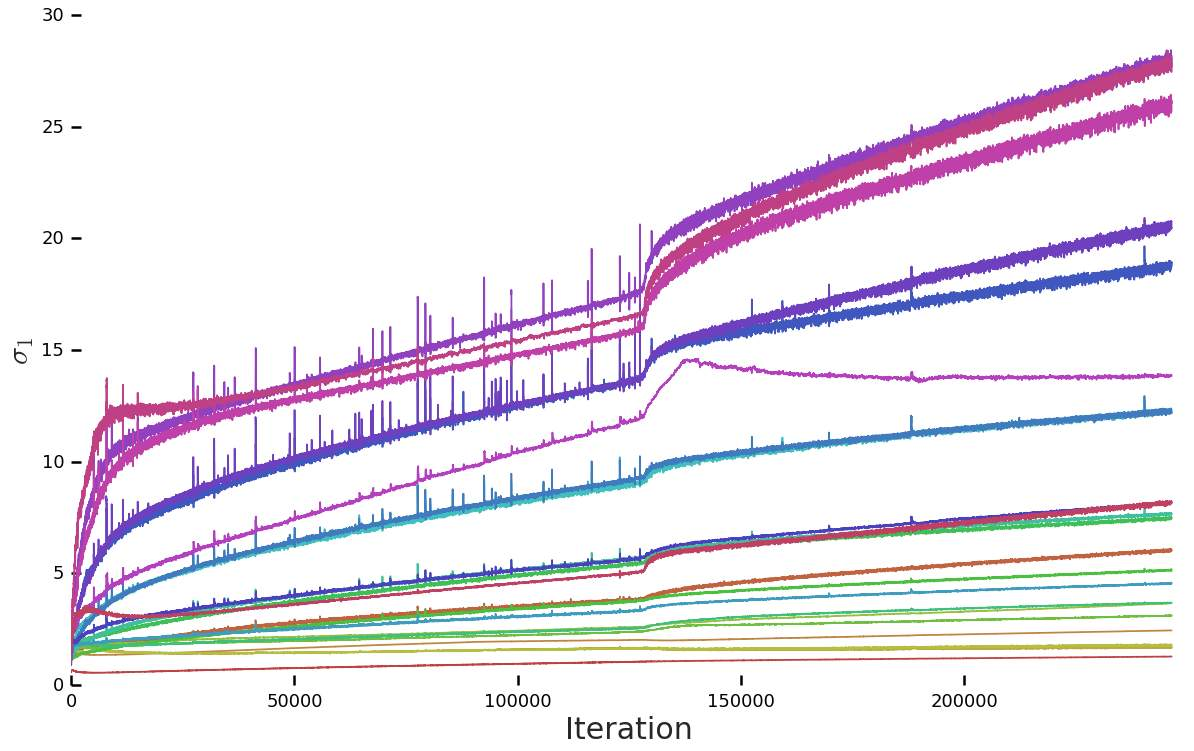
\includegraphics[width=0.48\textwidth]{images/1506681_GSR2_1/DSV1.jpg}}{(c) $\sigma_1$} & 
\subf{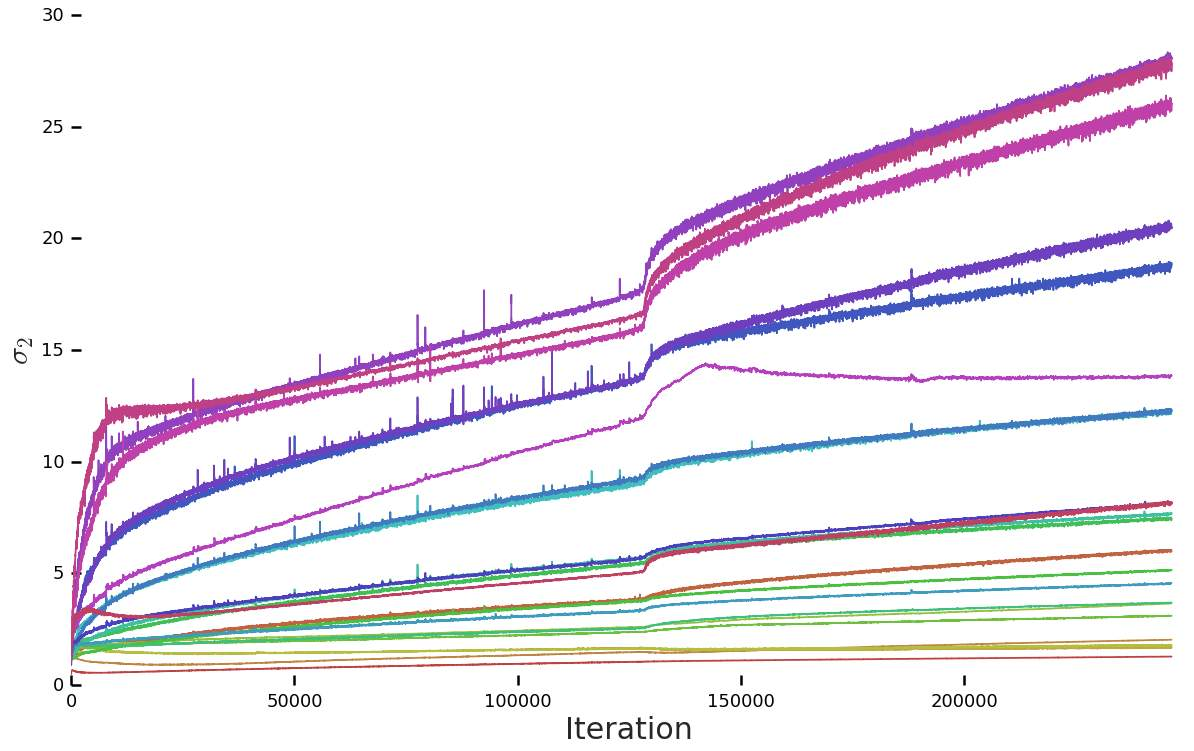
\includegraphics[width=0.48\textwidth]{images/1506681_GSR2_1/DSV2.jpg}}{(d) $\sigma_2$} \\
\end{tabular}
\caption{\discr{} training statistics with $\sigma_0$ in \gen{} regularized towards 1. Collapse occurs after 125000 iterations.}
\label{D_spectra_regsigma}
\end{figure}



% R1GP bois
\begin{figure}[htbp]
\centering
\setlength{\tabcolsep}{1pt}
\begin{tabular}{cc}
\subf{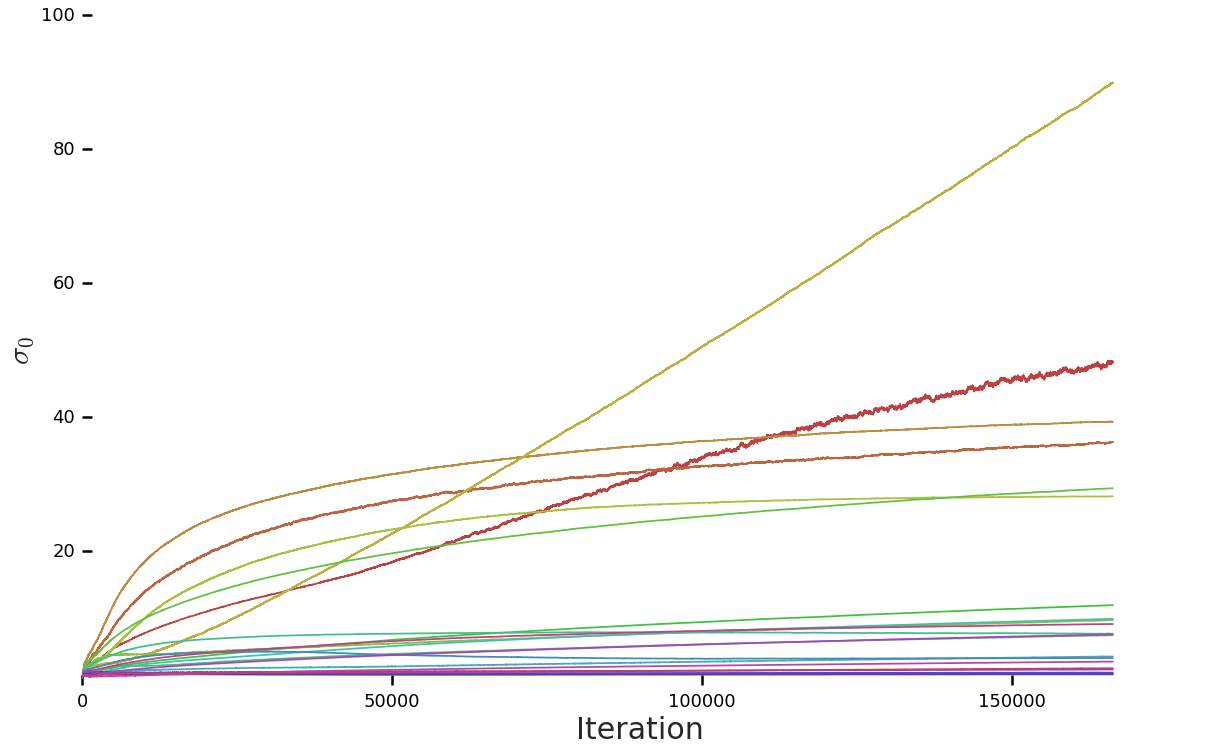
\includegraphics[width=0.48\textwidth]{images/1519233_R1GP5/GSV0.jpg}}{(a) $\sigma_0$ } & 
\subf{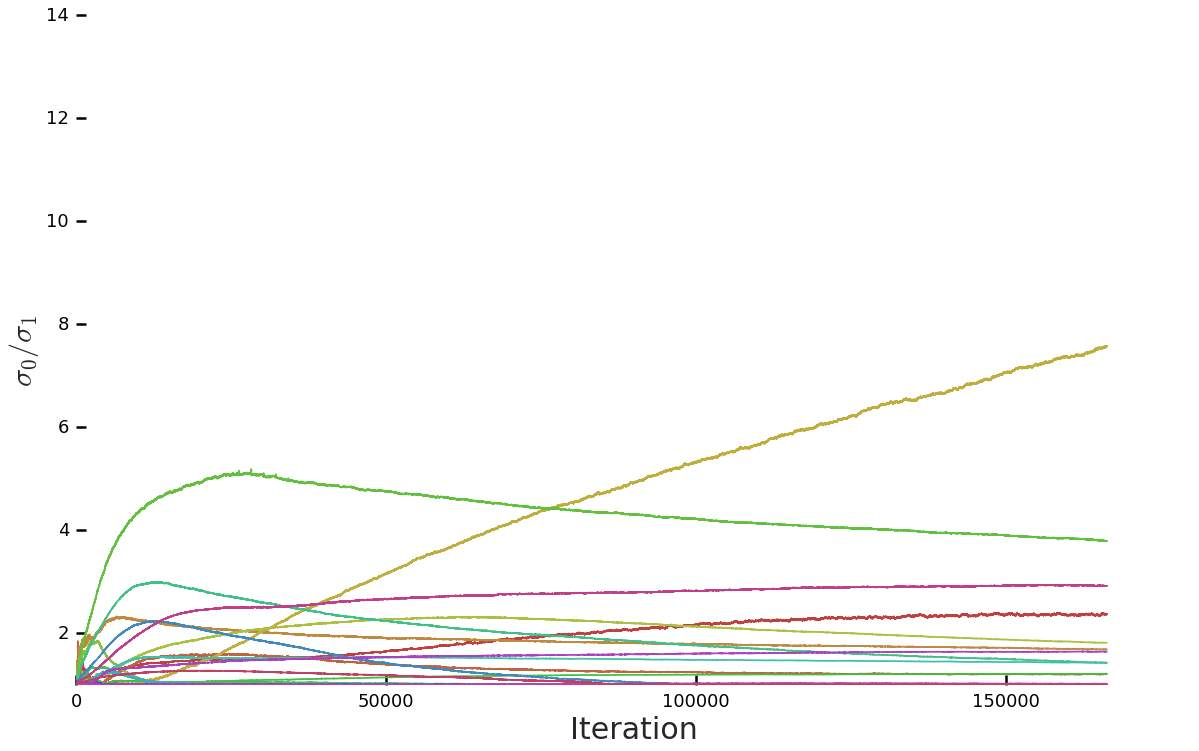
\includegraphics[width=0.48\textwidth]{images/1519233_R1GP5/GSVR.jpg}}{(b) $\frac{\sigma_0}{\sigma_1}$ } \\
\subf{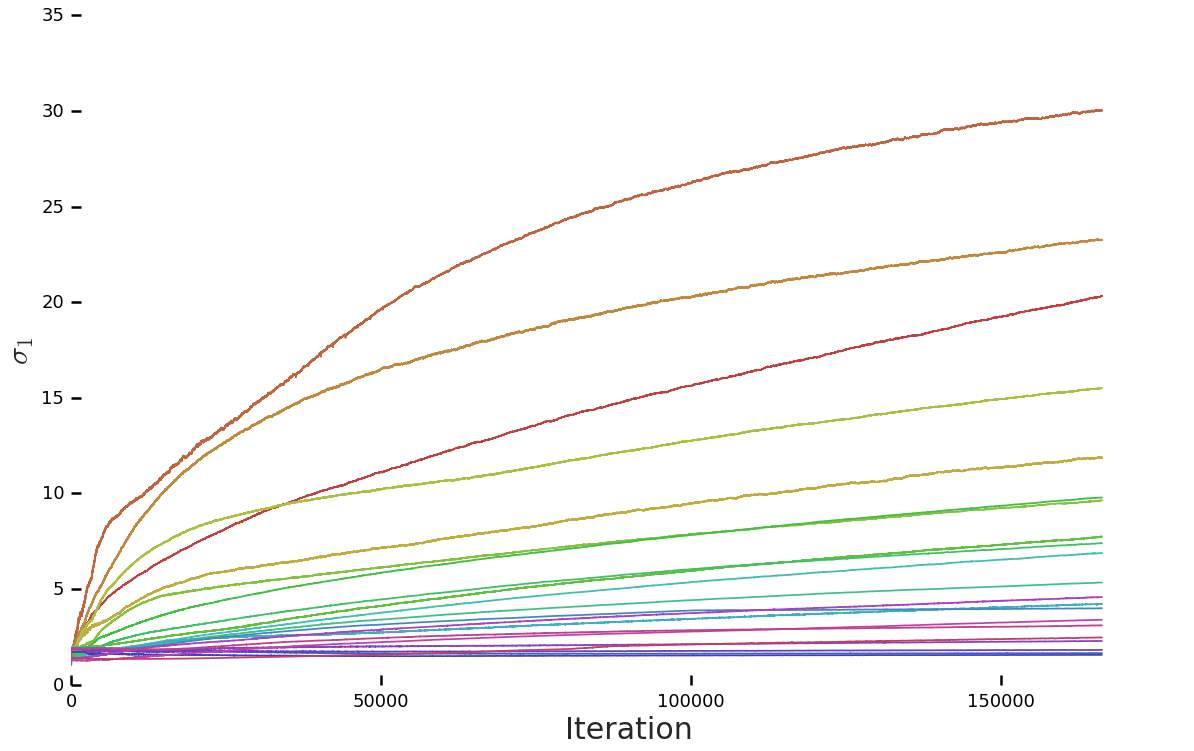
\includegraphics[width=0.48\textwidth]{images/1519233_R1GP5/GSV1.jpg}}{(c) $\sigma_1$} & 
\subf{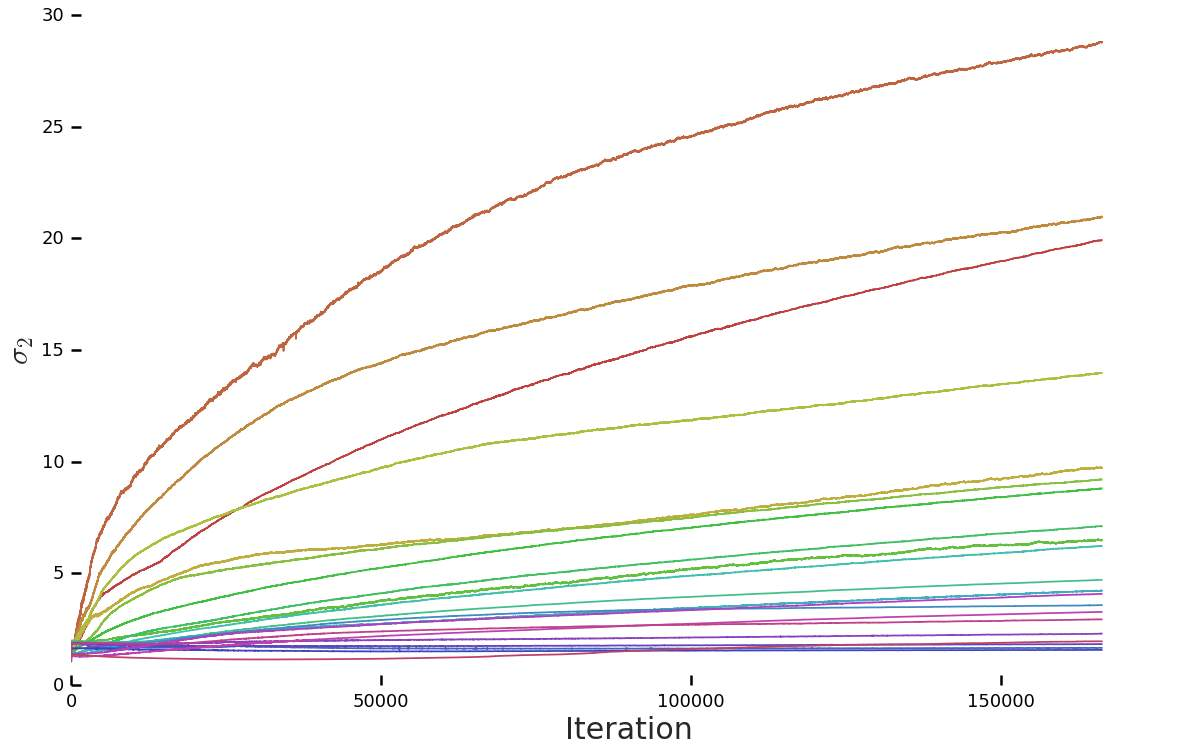
\includegraphics[width=0.48\textwidth]{images/1519233_R1GP5/GSV2.jpg}}{(d) $\sigma_2$} \\
\end{tabular}
\caption{\gen{} training statistics with an R1 Gradient Penalty of strength 10 on \discr{}. This model does not collapse, but only reaches a maximum IS of 55.}
\label{G_spectra_R1GP5}
\end{figure}

\begin{figure}[htbp]
\centering
\setlength{\tabcolsep}{1pt}
\begin{tabular}{cc}
\subf{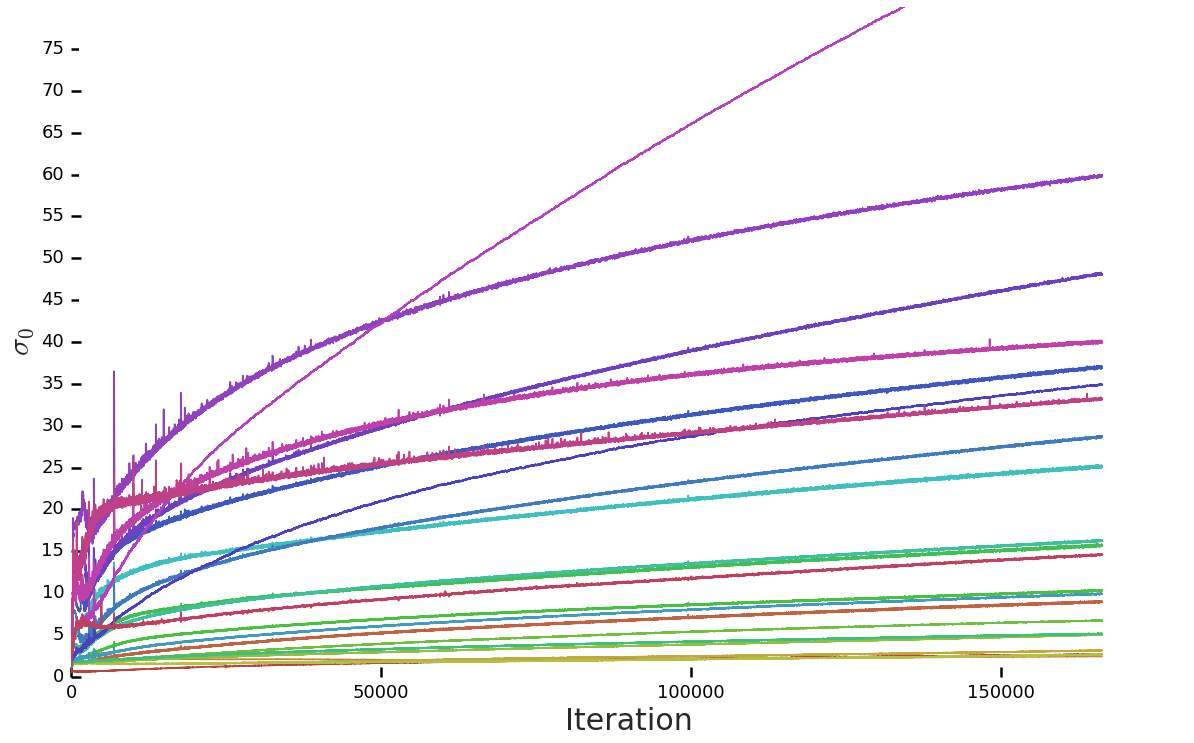
\includegraphics[width=0.48\textwidth]{images/1519233_R1GP5/DSV0.jpg}}{(a) $\sigma_0$ } & 
\subf{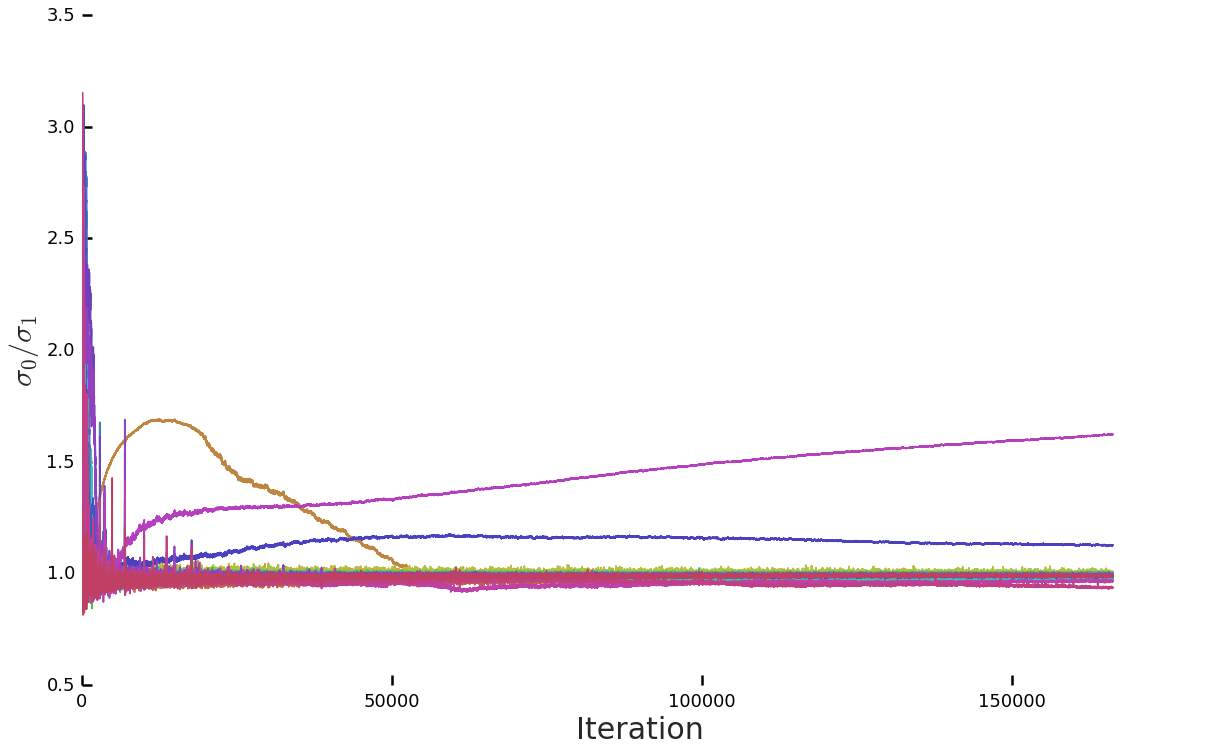
\includegraphics[width=0.48\textwidth]{images/1519233_R1GP5/DSVR.jpg}}{(b) $\frac{\sigma_0}{\sigma_1}$ } \\
\subf{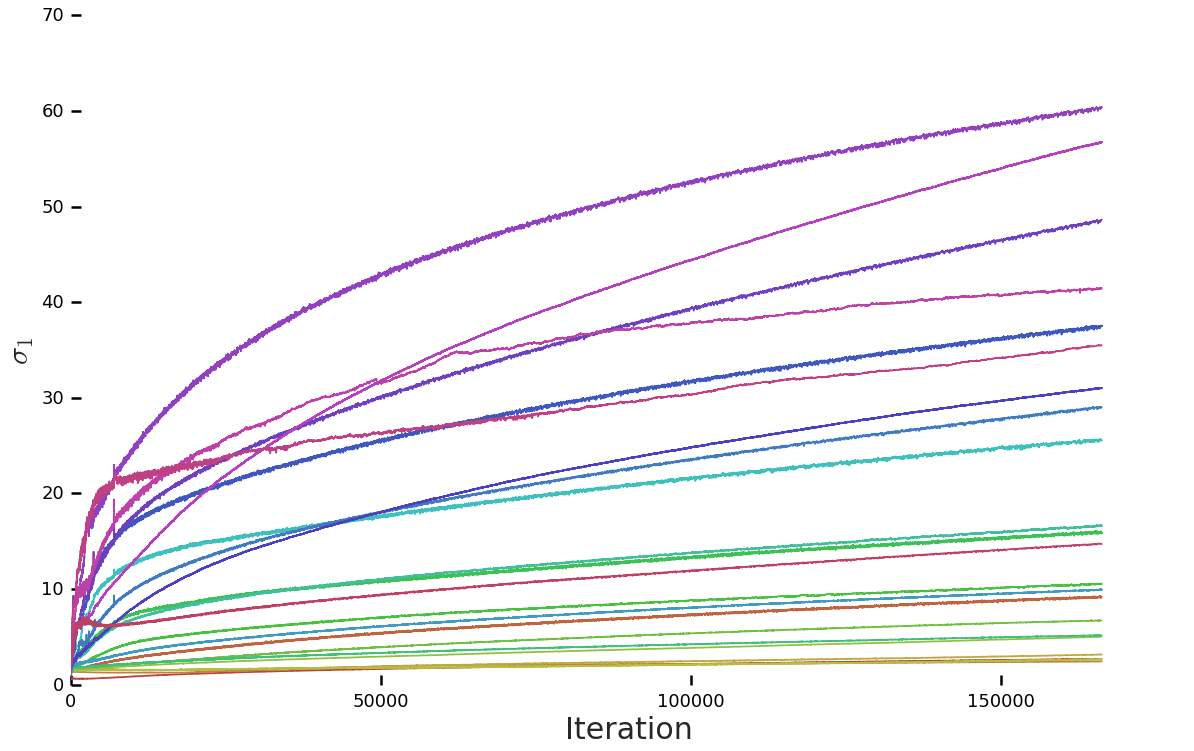
\includegraphics[width=0.48\textwidth]{images/1519233_R1GP5/DSV1.jpg}}{(c) $\sigma_1$} & 
\subf{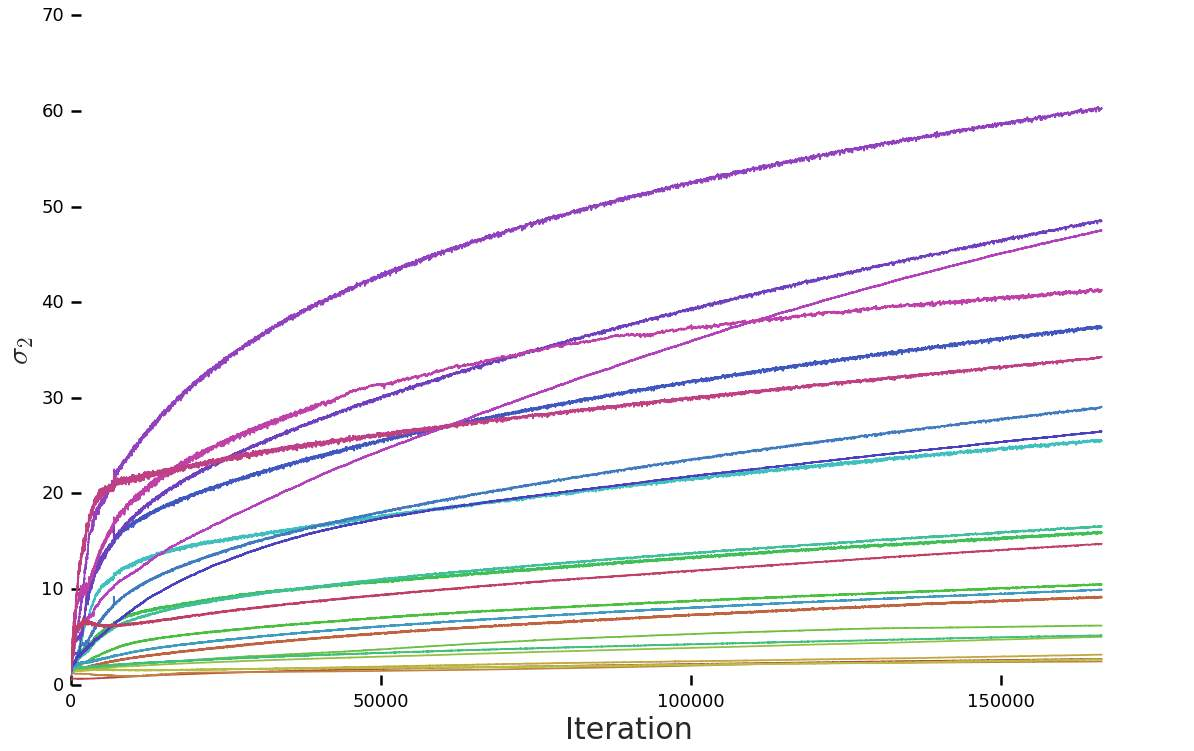
\includegraphics[width=0.48\textwidth]{images/1519233_R1GP5/DSV2.jpg}}{(d) $\sigma_2$} 
\end{tabular}
\caption{\discr{} training statistics with an R1 Gradient Penalty of strength 10 on \discr{}. This model does not collapse, but only reaches a maximum IS of 55.}
\label{D_spectra_R1GP5}
\end{figure}


% Dropout bois
\begin{figure}[htbp]
\centering
\setlength{\tabcolsep}{1pt}
\begin{tabular}{cc}
\subf{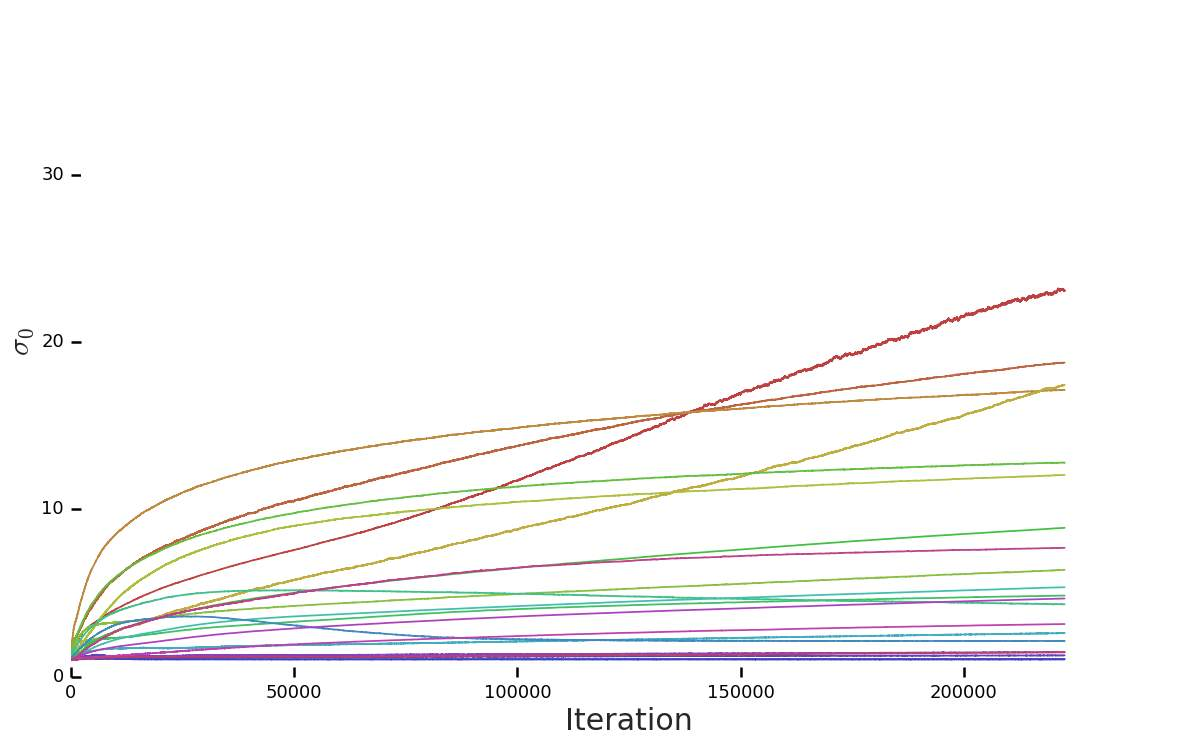
\includegraphics[width=0.48\textwidth]{images/1576139_dropout0.2/GSV0.jpg}}{(a) $\sigma_0$ } & 
\subf{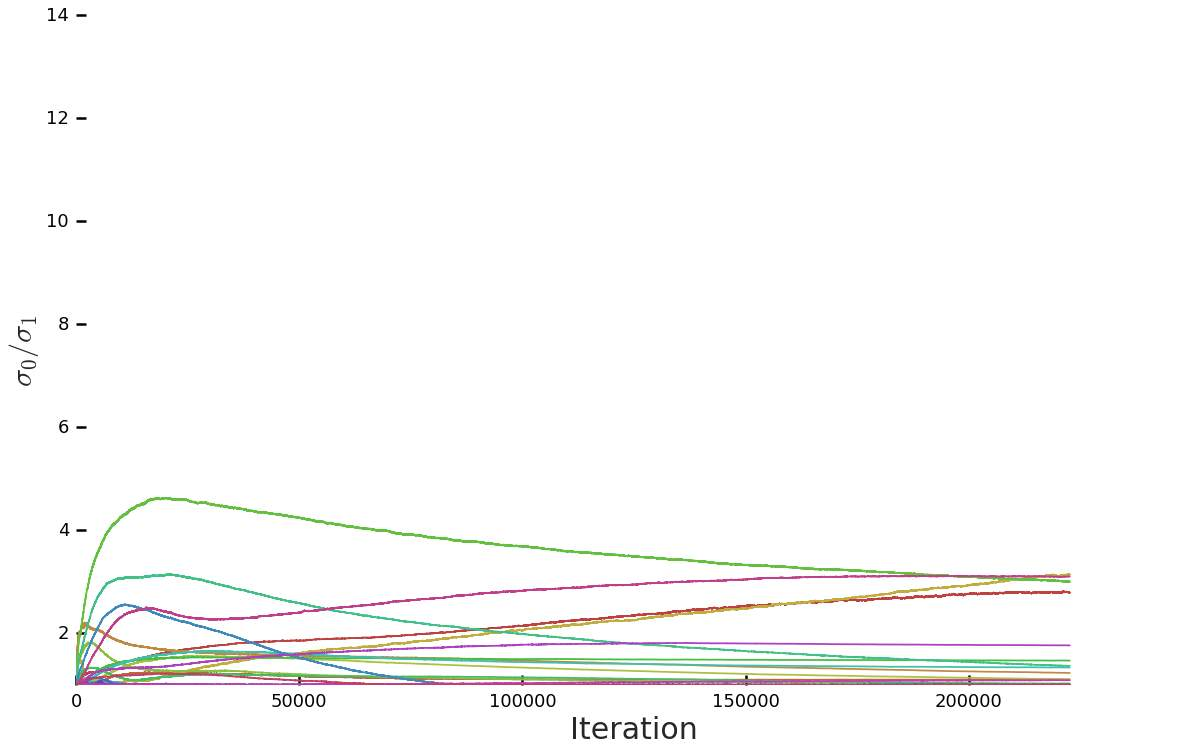
\includegraphics[width=0.48\textwidth]{images/1576139_dropout0.2/GSVR.jpg}}{(b) $\frac{\sigma_0}{\sigma_1}$ } \\
\subf{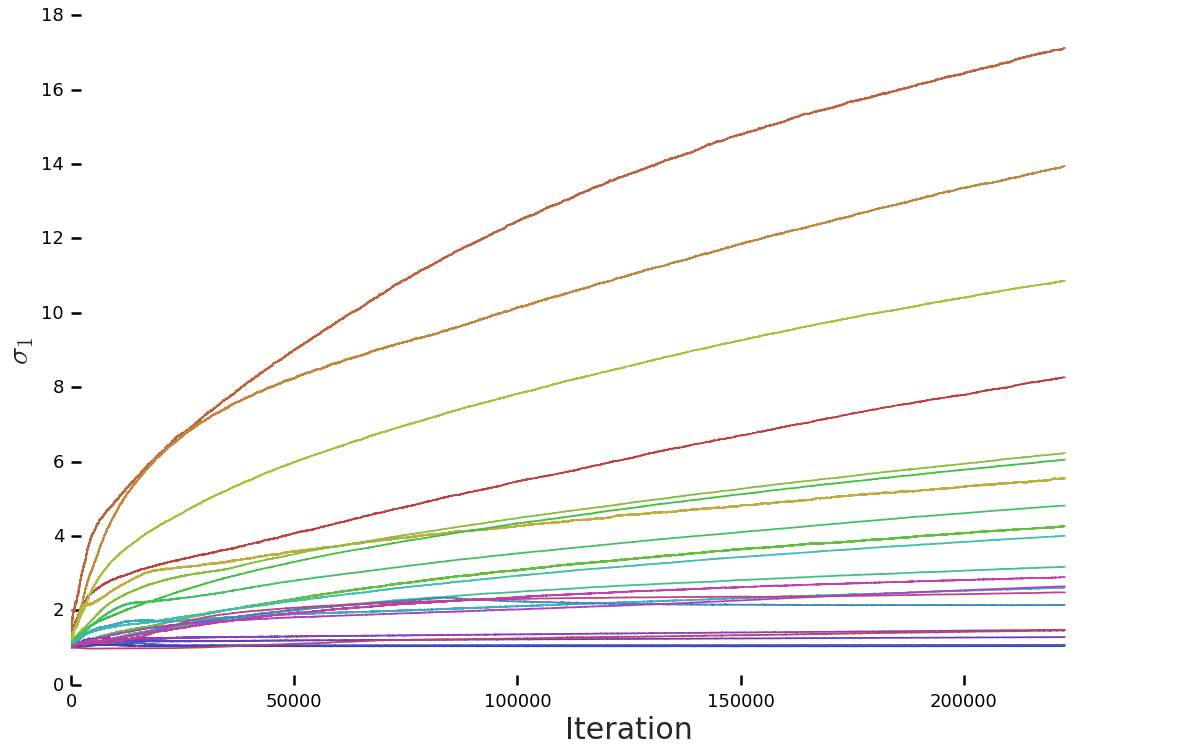
\includegraphics[width=0.48\textwidth]{images/1576139_dropout0.2/GSV1.jpg}}{(c) $\sigma_1$} & 
\subf{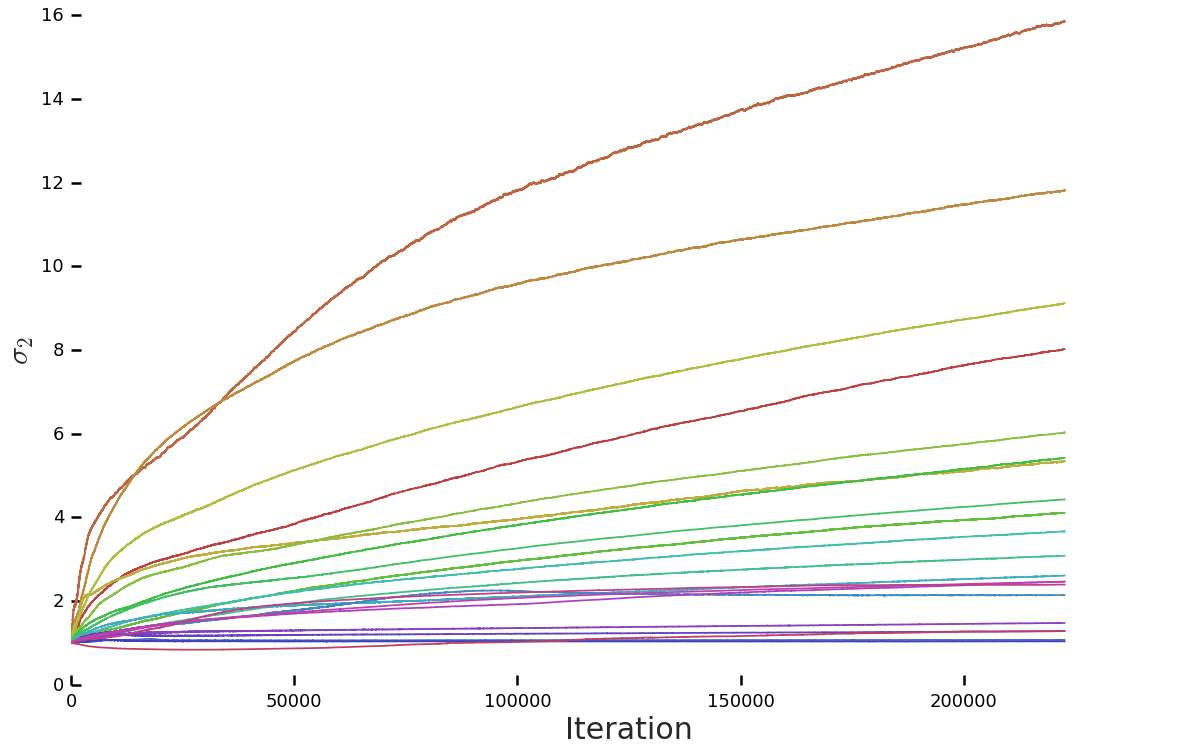
\includegraphics[width=0.48\textwidth]{images/1576139_dropout0.2/GSV2.jpg}}{(d) $\sigma_2$}
\end{tabular}
\caption{\gen{} training statistics with Dropout (keep probability 0.8) applied to the last feature layer of \discr{}. This model does not collapse, but only reaches a maximum IS of 70.}
\label{G_spectra_dropout0.2}
\end{figure}

\begin{figure}[htbp]
\centering
\setlength{\tabcolsep}{1pt}
\begin{tabular}{cc}
\subf{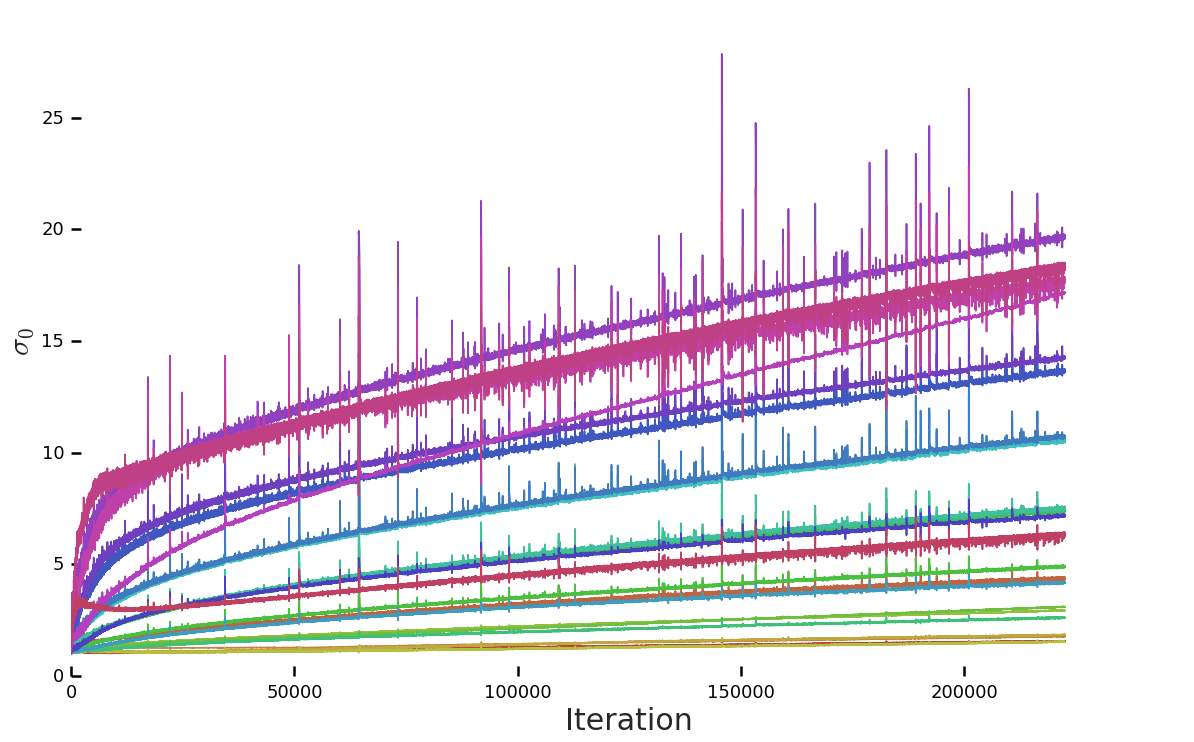
\includegraphics[width=0.48\textwidth]{images/1576139_dropout0.2/DSV0.jpg}}{(a) $\sigma_0$ } & 
\subf{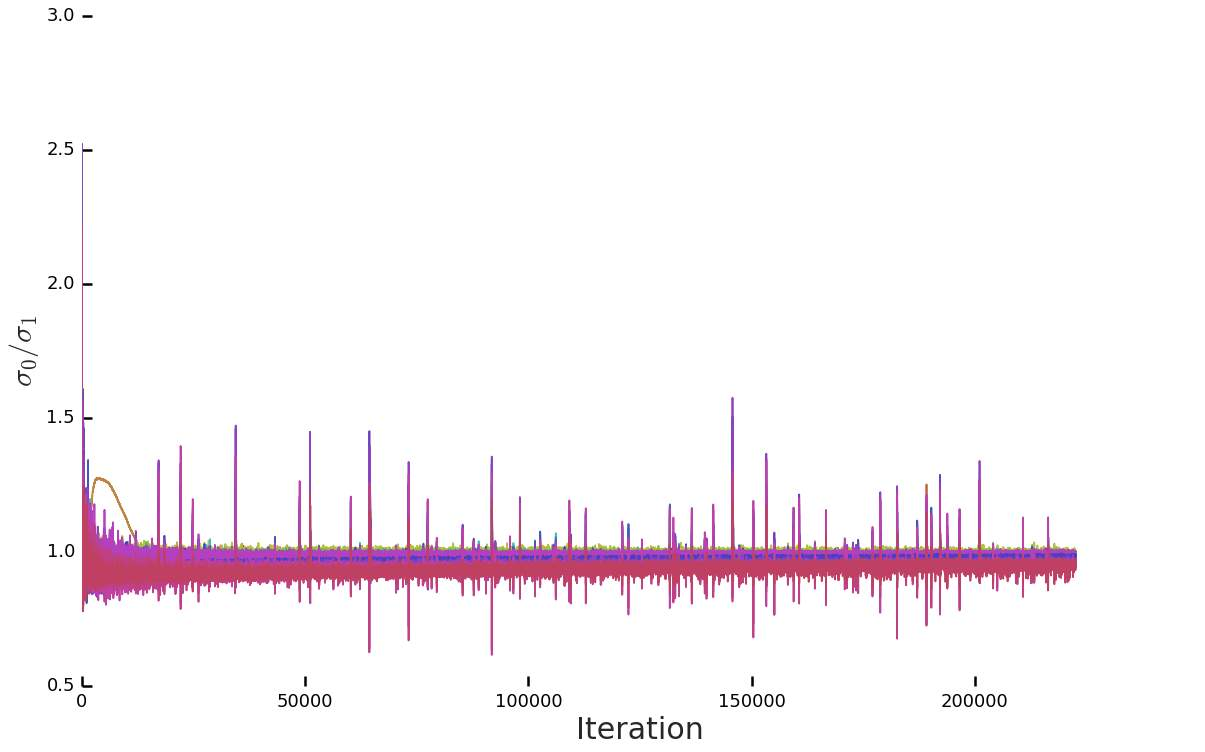
\includegraphics[width=0.48\textwidth]{images/1576139_dropout0.2/DSVR.jpg}}{(b) $\frac{\sigma_0}{\sigma_1}$ } \\
\subf{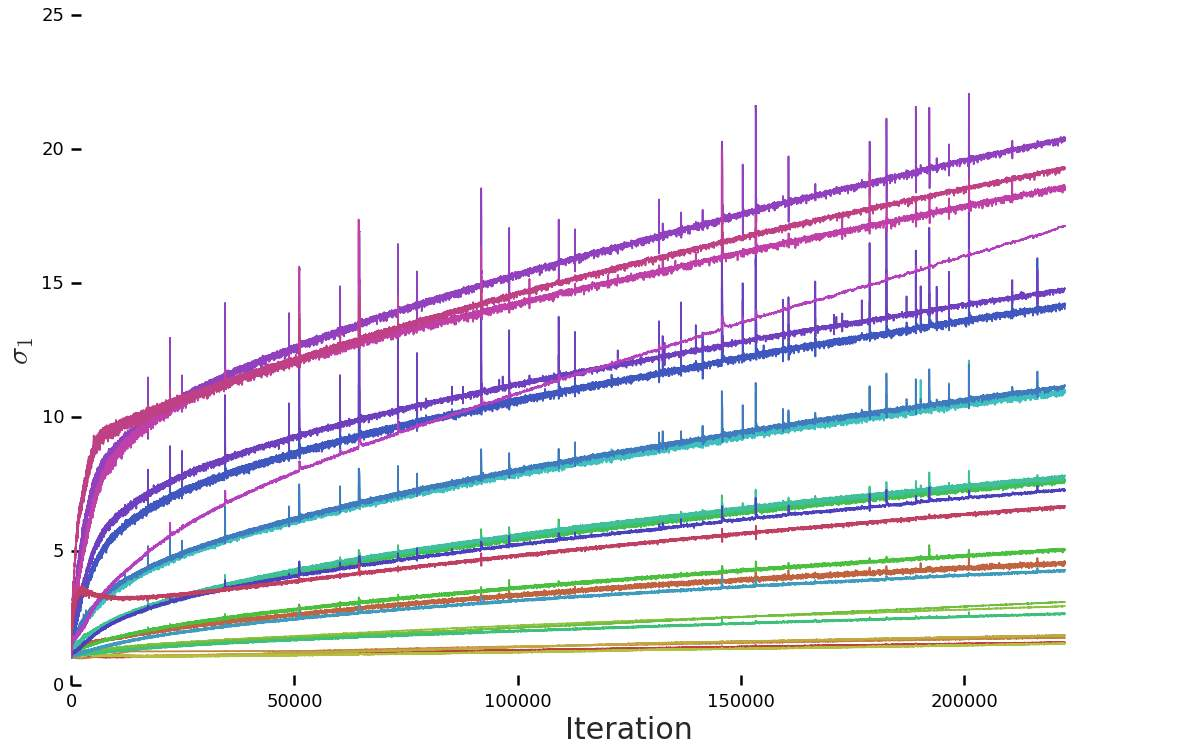
\includegraphics[width=0.48\textwidth]{images/1576139_dropout0.2/DSV1.jpg}}{(c) $\sigma_1$} & 
\subf{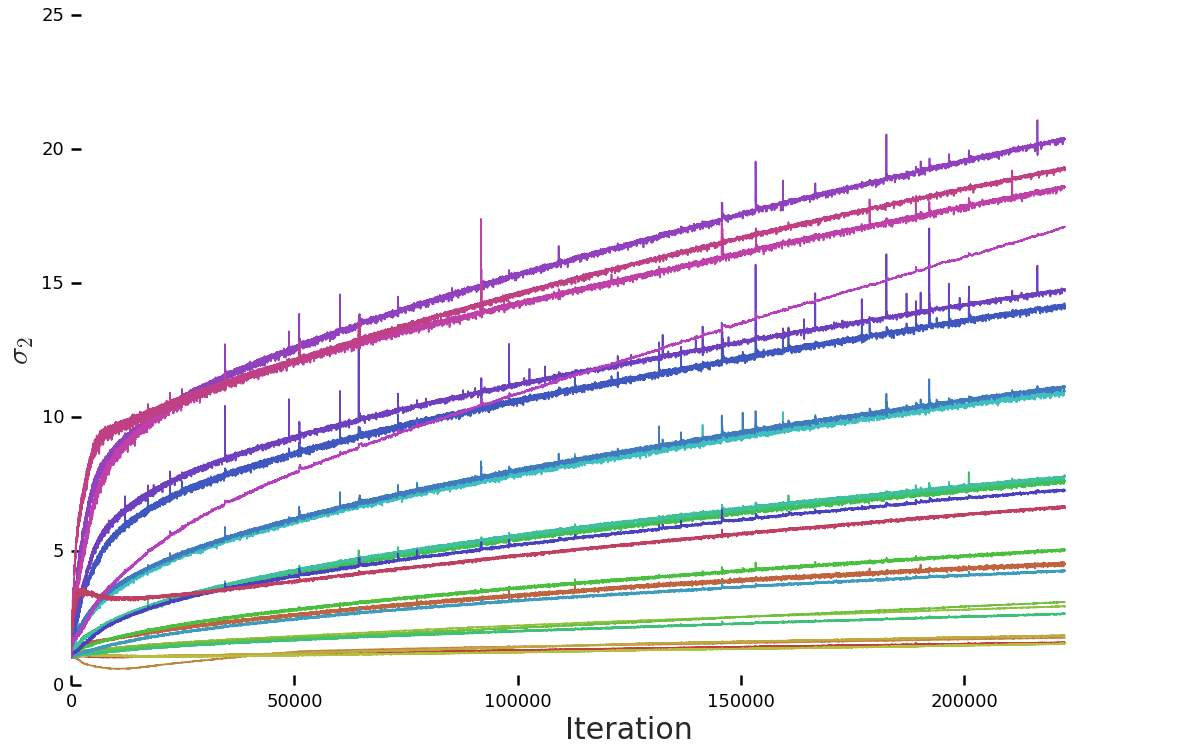
\includegraphics[width=0.48\textwidth]{images/1576139_dropout0.2/DSV2.jpg}}{(d) $\sigma_2$} \end{tabular}
\caption{\discr{} training statistics with Dropout (keep probability 0.8) applied to the last feature layer of \discr{}. This model does not collapse, but only reaches a maximum IS of 70.}
\label{D_spectra_dropout0.2}
\end{figure}



\begin{figure}[htbp]
\centering
\setlength{\tabcolsep}{1pt}
\begin{tabular}{cc}
\subf{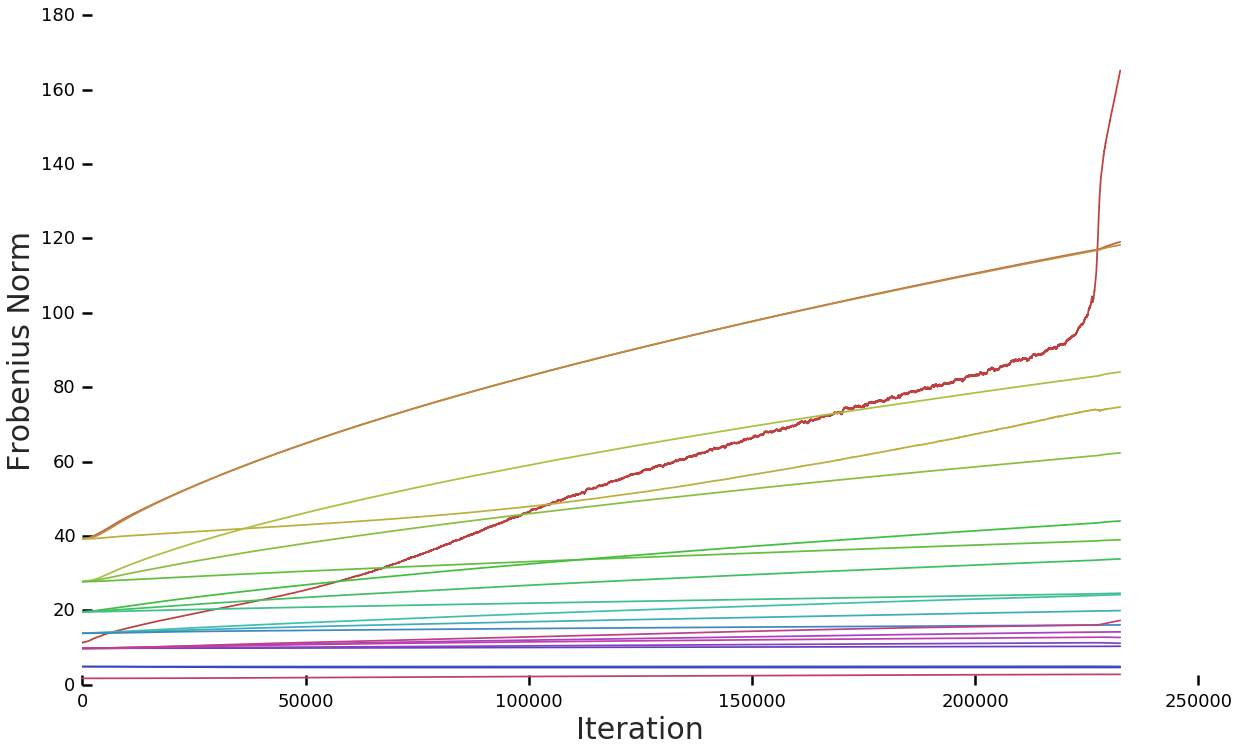
\includegraphics[width=0.48\textwidth]{images/1535537/GFROB.jpg}}{(a) \gen{} $\|W\|_2$} &
\subf{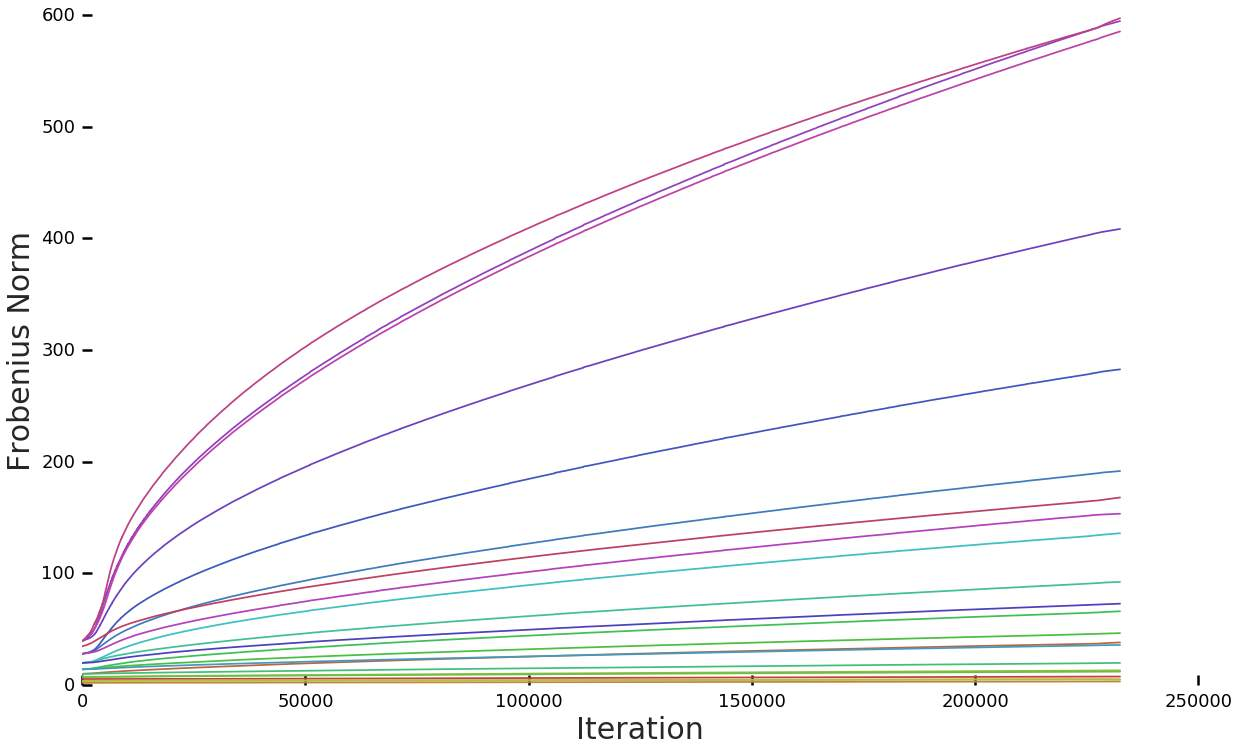
\includegraphics[width=0.48\textwidth]{images/1535537/DFROB.jpg}}{(b) \discr{} $\|W\|_2$} \\
\subf{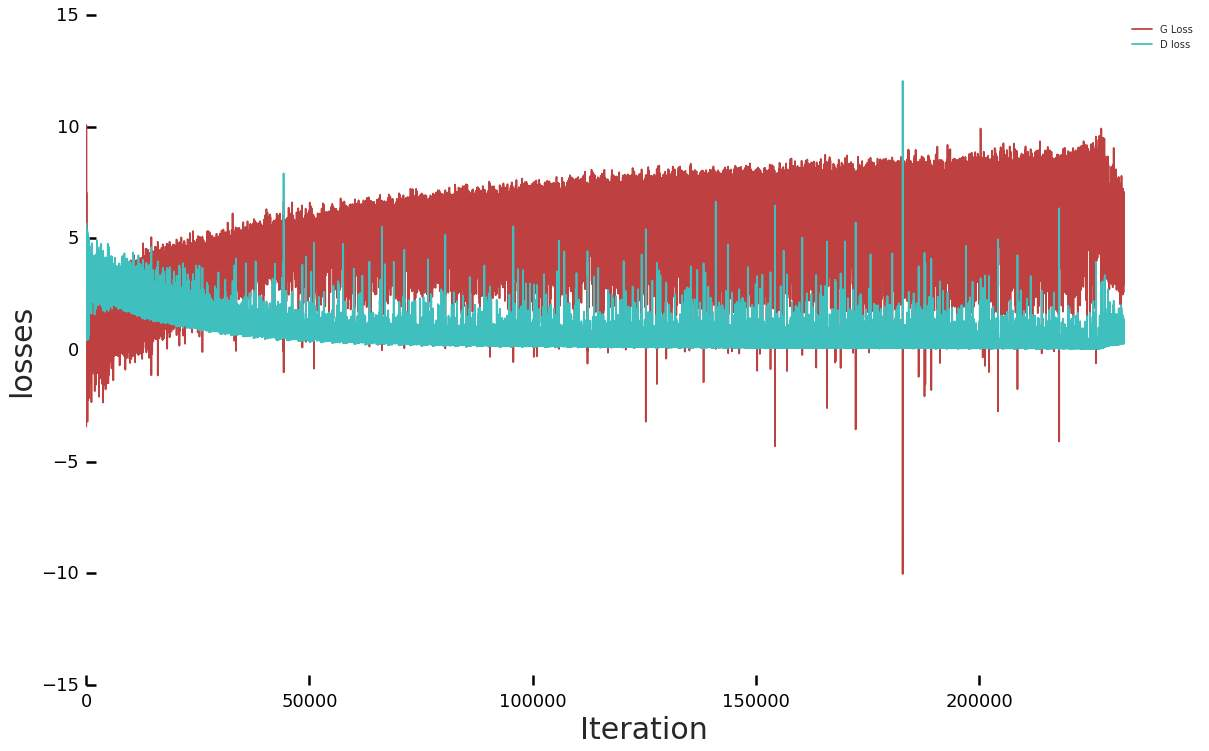
\includegraphics[width=0.48\textwidth]{images/1535537/losses.jpg}}{(c) losses} &
\subf{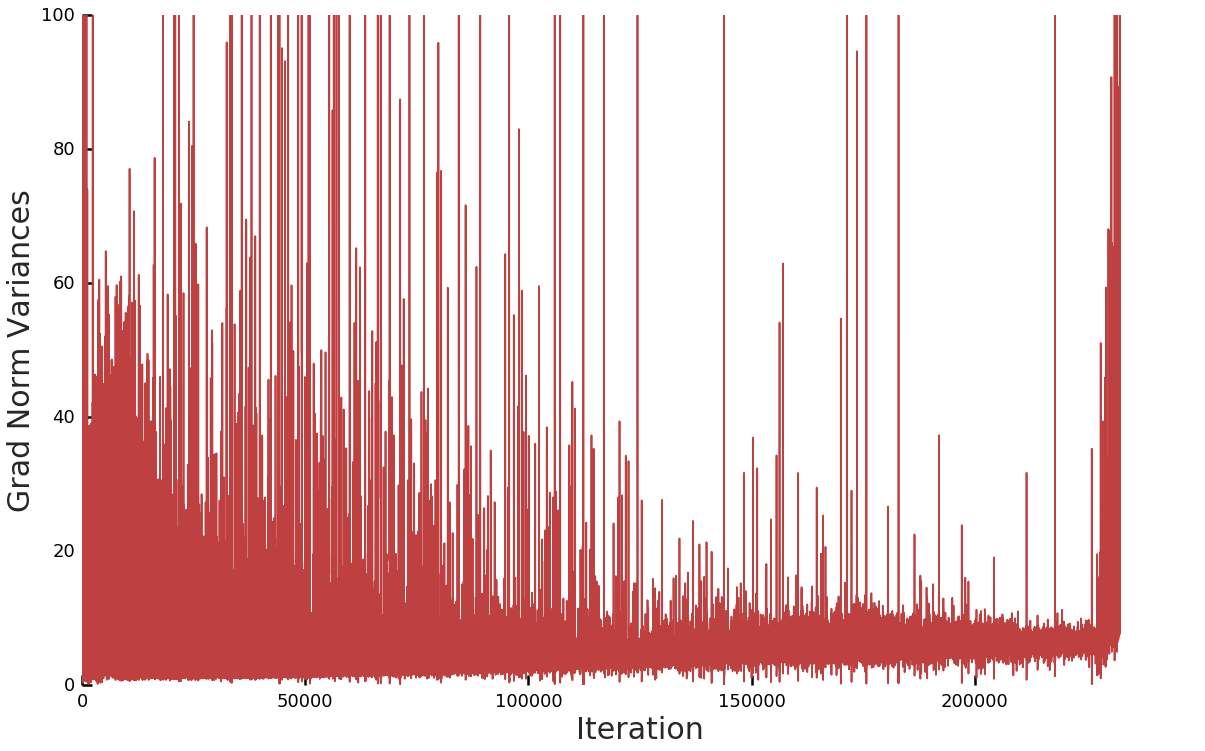
\includegraphics[width=0.48\textwidth]{images/1535537/gradnormvars.jpg}}{(d) Variance of all gradient norms in \gen{} and \discr{}}
\end{tabular}
\caption{Additional training statistics for a typical model without special modifications. Collapse occurs after 200000 iterations.}
\label{additional_stats_vanilla}
\end{figure}


\begin{figure}[htbp]
\centering
\setlength{\tabcolsep}{1pt}
\begin{tabular}{cc}
\subf{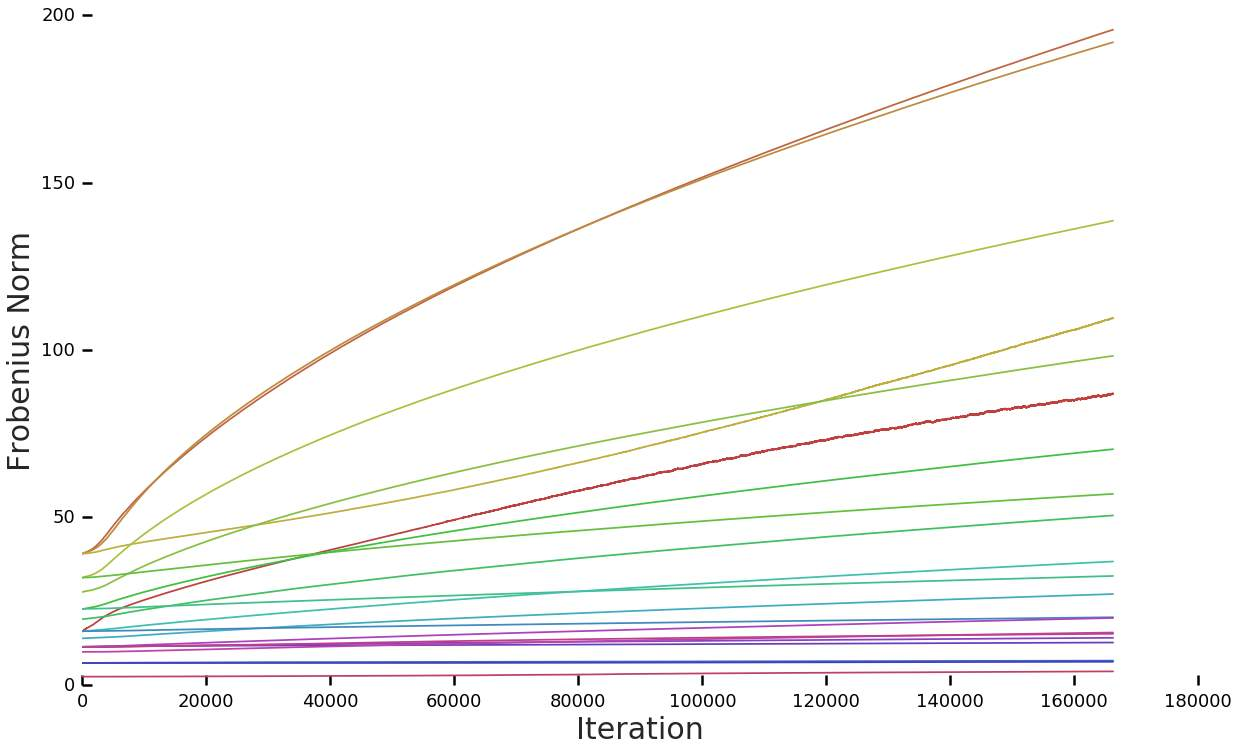
\includegraphics[width=0.48\textwidth]{images/1519233_R1GP5/GFROB.jpg}}{(a) \gen{} $\|W\|_2$} & 
\subf{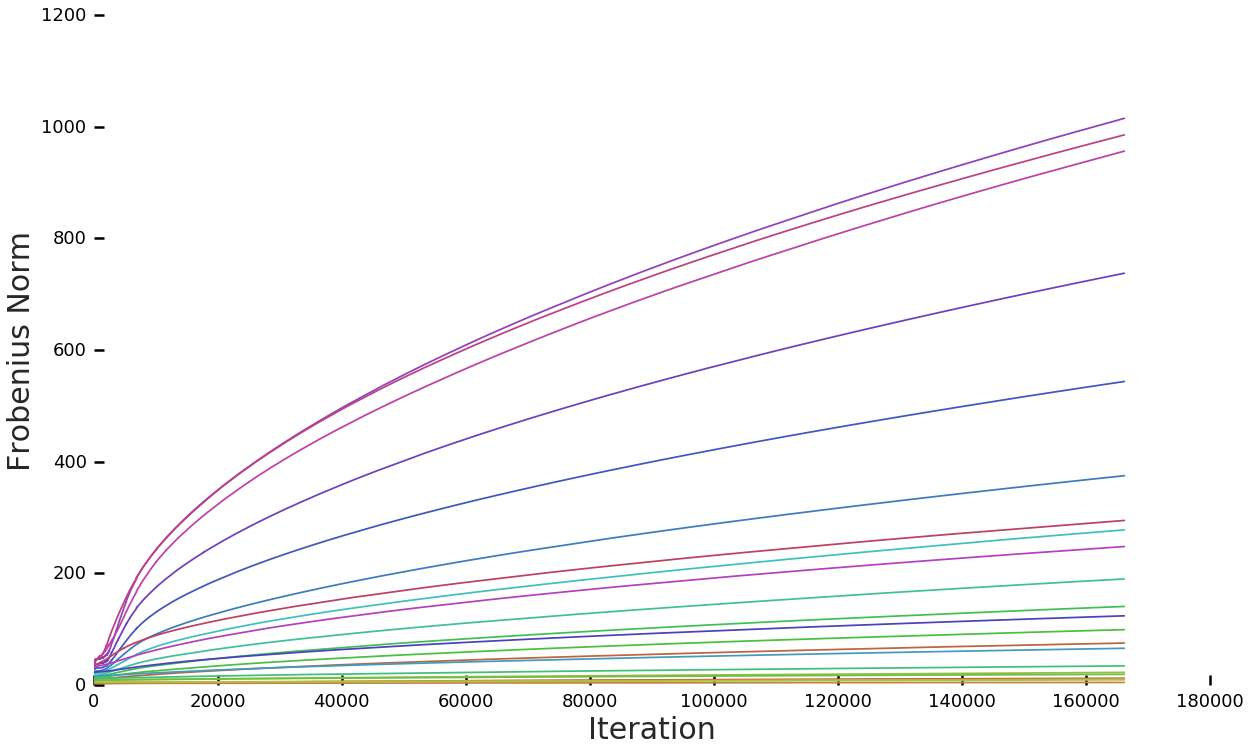
\includegraphics[width=0.48\textwidth]{images/1519233_R1GP5/DFROB.jpg}}{(b) \discr{} $\|W\|_2$} \\ 
\subf{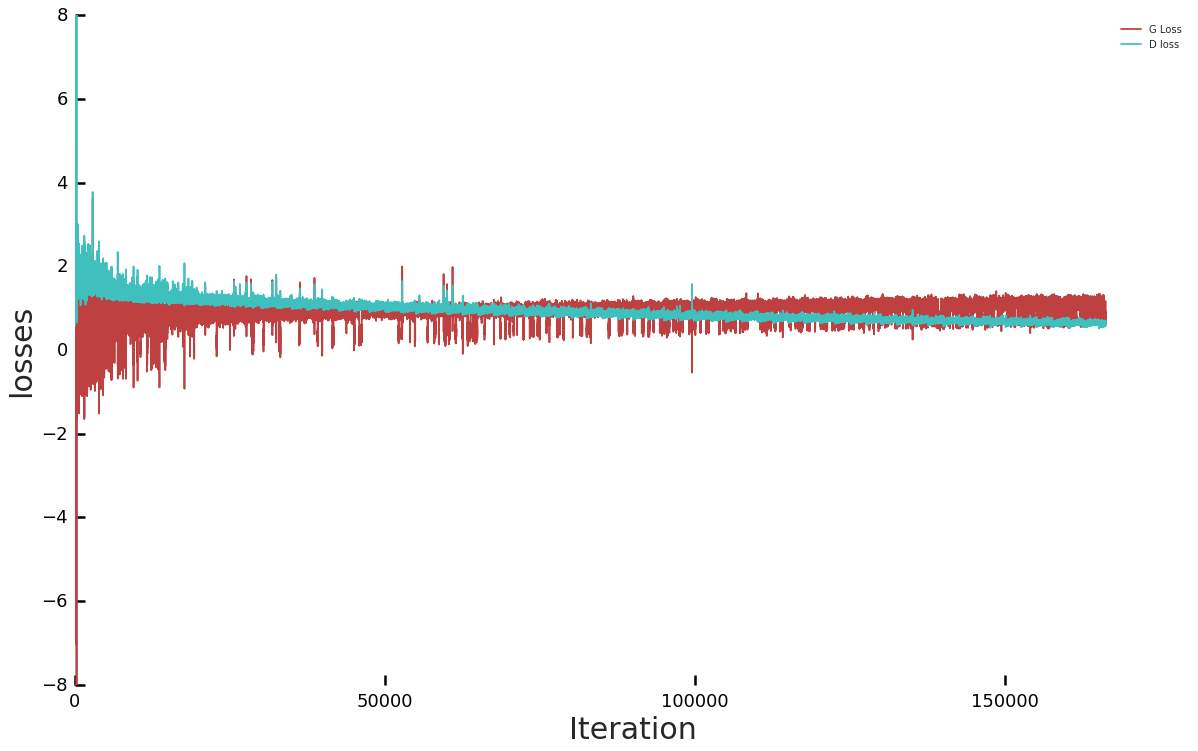
\includegraphics[width=0.48\textwidth]{images/1519233_R1GP5/losses.jpg}}{(c) losses} &
\subf{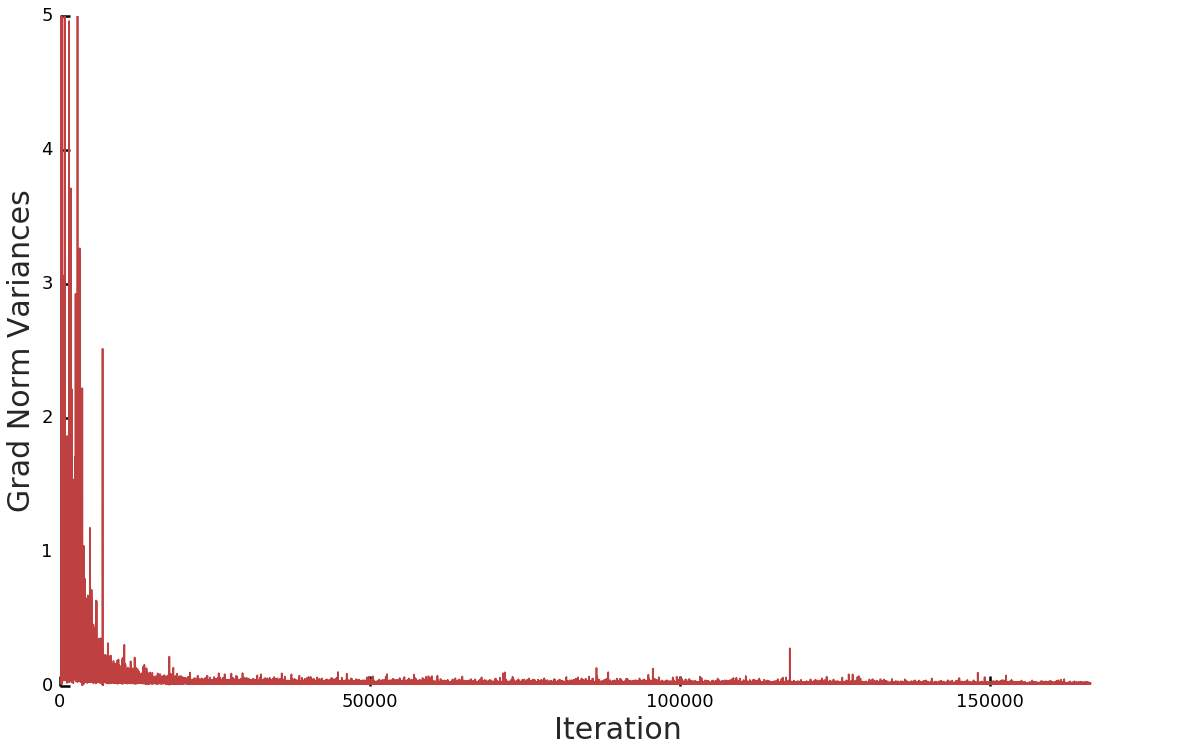
\includegraphics[width=0.48\textwidth]{images/1519233_R1GP5/gradnormvars.jpg}}{(d) Variance of all gradient norms in \gen{} and \discr{}}
\end{tabular}
\caption{Additional training statistics with an R1 Gradient Penalty of strength 10 on \discr{}. This model does not collapse, but only reaches a maximum IS of 55.}
\label{additional_stats_R1GP10}
\end{figure}

\clearpage